\documentclass[12pt]{article}
\usepackage[utf8]{inputenc}
\usepackage[T1]{fontenc}
\usepackage{amsmath}
\usepackage{amsfonts}
\usepackage{amssymb}
\usepackage{mhchem}
\usepackage{stmaryrd}
\usepackage{xcolor}
\newtheorem{remark}{Remark}
\usepackage{graphicx}
\usepackage{tikz}
\usetikzlibrary{arrows.meta}

\newtheorem{theorem}{Theorem}

\newtheorem{condth}{Condition}
\renewcommand*{\thecondth}{\Roman{condth}}
\newenvironment{condition}[2][]{\renewcommand{\thecondth}{#2}\begin{condth}[#1]\label{#2}}{\end{condth}\renewcommand{\thecondth}{\Roman{condth}}}


\title{A variational principle for non-conservative dynamics}
\author{TBD }

\begin{document}
\maketitle

\begin{abstract}
    TBD
\end{abstract}

\section{Introduction}

TBD

TODO: state that all objects are assumed smooth. Then remove mention of differentiability and smoothness throughout

\begin{condition}[Smoothness]{SM}
	All geometric objects are assumed smooth.
\end{condition}

\begin{condition}[Classical states in dynamical variables]{CSD}
	The state \linebreak space of a classical system with $n$ independent degrees of freedom (DOF) is represented by position and conjugate momentum. That is, given a set of $n$ position variables $q^i$, we can find a set of $n$ conjugate momentum variables $p_i$ such that each state is identified by position and momentum $(q^i,p_j) \in \mathbb{R}^{2n}$. Moreover, the count of configurations\footnote{By \emph{configuration} we mean the position-momentum pair for a single DOF.} for a DOF is given by $\int_{\Sigma} \omega = \int_{\Sigma} \sum_i dq^i dp_i$ with $\omega = \sum_i dq^i \wedge dp_i$. The count of states is given by the Liouville measure $\int_U \omega^n / n! = \int_U \prod_i dq^i dp_i$. 
\end{condition}

\begin{condition}[Classical states in kinematic variables]{CSK}
	The state \linebreak space of a classical system with $n$ independent degrees of freedom (DOF) is represented by position and velocity. That is, given a set of $n$ position variables $x^i$, we can find a set of $n$ velocity variables $v^i$ such that each state is identified by position and velocity $(x^i,v^j) \in \mathbb{R}^{2n}$. Moreover, over time evolution, $v^i = d_t x^i$.
\end{condition}

\begin{theorem}
	Consider the following conditions:
	\begin{description}
		\item[TE-EOM] (Equations of motion) The evolution obeys explicit equations of motion. That is, $d_t \gamma^a(t) = S^a$.
		\item [TE-FLUX] (Evolution kills the flux) The evolution kills the flux of configuration. That is, there exists a configuration flux form $w_{ab}$ such that $w_{ab}|_{(q^i,p_j)}=\omega_{ab}$ and $d_t \gamma^a(t) w_{ab}=0$;
		\item [TE-STFL] (Principle of stationary flux in phase space) The evolution between two given positions is the one that renders the flux around it stationary. That is, there exists a flux functional $\phi[\Sigma]=\int_{\Sigma} w$ such that $w_{ab}|_{(q^i,p_j)}=\omega_{ab}$ and $\delta \phi[\Sigma_{\gamma, \epsilon \eta}]=0$ where $\Sigma_{\gamma, \epsilon \eta}$ is the surface between the path $\gamma^a$ and its variation $\gamma^a + \epsilon \eta^a$.
		\item [DI-SYMP] (Symplectomorphism) The evolution preserves the configuration count and DOF independence. That is, $d_t \omega = 0$.
		\item [DI-STAC] (Principle of stationary action in phase space) The evolution between two given positions is the one for which the phase space action is stationary. That is, there exists an action functional $\mathcal{A}_H[\gamma] = \int (p_i d_t q^i -H)dt$ such that  $\delta \mathcal{A}_H[\gamma] = 0$.
		\item[KE](Kinematic Equivalence)
		The system can be equivalently described in dynamic and kinematic variables. That is, there is an invertible map between position and momentum $(q^i, p_i)$ and position and velocity $(x^i, v^i)$.
		\item [KE-STFL] (Principle of stationary flux) The evolution between two given positions is the one that renders the flux around it stationary. That is, there exists a flux action functional $\mathcal{FA}[x^i_a(t), x^i_b(t)] =$ \linebreak $\int \mathrm{FL}(x^i_a(t), d_t x^i_a(t), x^i_b(t), d_t x^i_b(t), t)dt$ where $\mathrm{FL}$ is a hyperregular flux Lagrangian such that  $\delta_b \mathcal{FA}[x^i(t),x^i(t)] = 0$.
		\item [KEDI-STFL] (Principle of stationary flux) The evolution between two given positions is the one that renders the additive flux around it stationary. That is, there exists a flux action functional $\mathcal{FA}[x^i_a(t), x^i_b(t)] =$  $\int \mathrm{FL}(x^i_a(t), d_t x^i_a(t), x^i_b(t), d_t x^i_b(t), t)dt$ where $\mathrm{FL}$ is an additive hyperregular flux Lagrangian such that  $\delta_b \mathcal{FA}[x^i(t),x^i(t)] = 0$.
		\item [KEDI-STAC] (Principle of stationary action) The evolution between two given positions is the one for which the action is stationary. That is, there exists an action functional $\mathcal{A}_L[x^i(t)] = \int L(x^i(t), d_t x^i(t), t)dt$ where $L$ is a hyperregular Lagrangian such that $\delta \mathcal{A}_L[x^i(t)] = 0$.
	\end{description}
	Correspondence across kinematic and dynamical variables: over \ref{SM}, \ref{CSD} \linebreak +KE+TE-EOM $\iff$ \ref{CSK}+KE-STFL $\impliedby$ \ref{CSD}+KE+DI-SYMP $\iff$ \ref{CSK}+KEDI-STFL.
	
	Characterizations of general and conservative dynamics in dynamical variables: over \ref{SM}+\ref{CSD}, TE-EOM $\iff$ TE-FLUX $\iff$ TE-STFL $\impliedby$ DI-SYMP $\iff$ DI-STAC.
	
	Characterization of general and conservative dynamics in kinematic variables: over \ref{SM}+\ref{CSK}, KE-STFL $\impliedby$ KEDI-STFL $\iff$ KEDI-STAC.
\end{theorem}

\section{Arbitrary dynamics in the extended phase space}

In this section we outline the theory for a classical dynamical system on the extended phase space. At each time, we have standard phase space with the geometry given by the count of configurations defined by the closed form $\omega_{ab}$. The dynamics in time, however, need not be conservative (i.e. Hamiltonian). The main result is the existence of a flux form $w_{ab}$ that characterizes the flux of configurations through a surface, and that the only direction that kills said flux is the displacement field $S^a$. That is, $v^a w_{ab} = 0$ if and only if $v^a = k S^a$ for some $k \in \mathbb{R}$.  

We consider a system as defined by classical mechanics, classed assumption (CST) for Classical STates, where each state is fully identified by position and conjugate momentum $(q^i,p_j) \in \mathbb{R}^{2n}$. Given a region $U \subseteq \mathbb{R}^{2n}$, the count of states is given by $\int_U \Omega = \int_U \omega^n / n! = \int_U \prod_i dq^i dp_i$. That is, the volume form $\Omega$ that defines the count of states locally is the product of the count of configuration for each degree of freedom (DOF) given by $\omega_{ab}$. In the context of Reverse Physics, this corresponds to the Infinitesimal Reducibility (IR) assumption (i.e the system can be thought as made of infinitesimal parts, or particles) and the INDependence of all degrees of freedom (IND).

Extending this setting with time, states are identified at a specific time using generalized coordinates $\xi^a = (q^i,p_i,t) \in \mathbb{R}^{2n+1}$. A path for the system is defined by a curve $\gamma^a(t) = (q^i(t), p_i(t), t)$, which tells us how the system evolves in time. Note that the time component has to match time itself, $\gamma^t(t) = t$, meaning that time plays a double role of coordinate (i.e. an element of $\xi^a$) and affine parameter (i.e. the parameter of the curve).

\begin{figure}[h]
    \centering
	% Requires \usepackage{tikz} and \usetikzlibrary{arrows.meta}.
% Cross-sections lie in parallel constant-time planes; time points right.
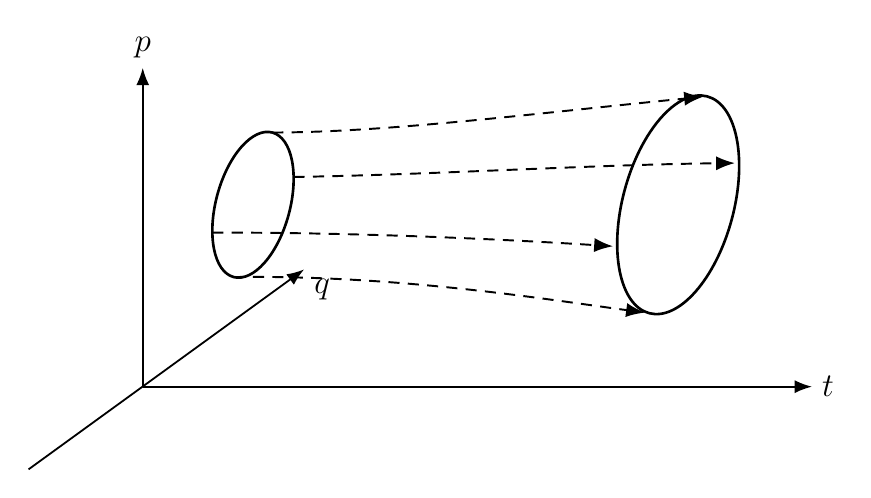
\begin{tikzpicture}[
    x=1cm,y=1cm,
    axis/.style={line width=0.65pt,-{Latex[length=2.2mm]}},
    section/.style={line width=0.95pt,line join=round},
    flow/.style={line width=0.7pt,dash pattern=on 4pt off 3pt,
                 -{Latex[length=2.4mm]},shorten >=1.5pt},
    every node/.style={font=\large}
]
    % The projected q and p directions span each cross-section.
    \draw[axis] (0,0) -- (8.5,0) node[right] {$t$};
    \draw[axis] (0,0) -- (0,4.05) node[above] {$p$};
    \draw[axis] (-1.45,-1.05) -- (2.05,1.49) node[below right] {$q$};

    % Four corresponding points on the initial and final boundaries.
    % The final section expands while keeping its centre at the same (q,p).
    \begin{scope}[shift={(1.40,2.31)},rotate=-15]
        \coordinate (aTop)    at (0,0.95);
        \coordinate (aRight)  at ({0.47*cos(30)},{0.95*sin(30)});
        \coordinate (aBottom) at (0,-0.95);
        \coordinate (aLeft)   at ({0.47*cos(210)},{0.95*sin(210)});
    \end{scope}
    \begin{scope}[shift={(6.80,2.31)},rotate=-15]
        \coordinate (bTop)    at (0,1.425);
        \coordinate (bRight)  at ({0.705*cos(30)},{1.425*sin(30)});
        \coordinate (bBottom) at (0,-1.425);
        \coordinate (bLeft)   at ({0.705*cos(210)},{1.425*sin(210)});
    \end{scope}

    % Evolution curves joining the two cross-sections.
    \draw[flow] (aTop)    .. controls (3.15,3.23) and (5.05,3.48) .. (bTop);
    \draw[flow] (aLeft)   .. controls (2.65,1.96) and (4.45,1.88) .. (bLeft);
    \draw[flow] (aRight)  .. controls (3.65,2.69) and (5.72,2.82) .. (bRight);
    \draw[flow] (aBottom) .. controls (3.20,1.42) and (5.05,1.12) .. (bBottom);

    % Regular tilted ellipses with smooth joins throughout.
    \draw[section,shift={(1.40,2.31)},rotate=-15]
        (0,0) ellipse[x radius=0.47,y radius=0.95];
    \draw[section,shift={(6.80,2.31)},rotate=-15]
        (0,0) ellipse[x radius=0.705,y radius=1.425];
\end{tikzpicture}

    \caption{Every two-dimensional surface at constant time is transported to another two-dimensional surface at constant time forming an evolution tube. The flux of configurations must be zero on the sides, therefore the net flux is the count of configurations at the end minus the count of configurations at the beginning. The dynamics is conservative if the flux over a closed surface is always zero, meaning that each evolution tube conserves the count of configurations and the independence of the degrees of freedom (i.e. mixed planes, like $(q^1,q^2)$, do not identify configurations for an independent DOF).}\label{evolutionTube}
\end{figure}

Assuming that we have a dynamical system that leaves probability densities well-defined throughout the evolution, there must be a displacement field $S^a(q^i,p_i,t)$ that tells how states evolve in time.\footnote{We will require the evolution to be differentiable in all parameters, leaving the exact physical meaning of that requirement for future work.} Therefore $\gamma^a(t)$ is an evolution of the system if and only if $d_t \gamma^a(t) = S^a(\gamma^a(t)) = S^a(q^i(t),p_i(t),t)$, which represents the equation of motion. In components, this becomes
\begin{equation}
    d_t \gamma^a(t) = \begin{bmatrix}
\dfrac{dq^i}{dt} \\[1em]
\dfrac{dp_i}{dt} \\[1em]
\dfrac{dt}{dt}
\end{bmatrix} = \begin{bmatrix}
S^{q^i}(q^i,p_i,t) \\[1em]
S^{p_i}(q^i,p_i,t) \\[1em]
S^{t}(q^i,p_i,t) 
\end{bmatrix}= S^a(q^i,p_i,t).
\end{equation}
Since $\gamma^t = t$, we must have that $S^t=1$.

We now want to characterize the flux of states, how the count of states flows in time. As described in Fig. \ref{evolutionTube}, if we start with a region $U$ at constant time, this will be mapped to a region $U'$ at a future time, forming an evolution tube where $U$ and $U'$ are the ends and the sides are evolution curves. The sides are always tangent to the displacement field $S^a$ and therefore they do not contribute to the flux. Given a generic hypersurface $U$, we are looking for a linear functional $\Phi(U) = \int_U W$ that must coincide with the state counting volume form at equal time, $W|_t = \Omega$ and must be zero along the flow, $W(S^a, \cdots) = 0$. This is enough to characterize the state flux form $W$.

In fact, all components with no time index will either be zero, if there are repetitions, or $\pm 1$ depending on orientation. For example,
\begin{equation}
    \begin{matrix}
        W_{q^1 p_1 q^2 p_2 \cdots q^n p_n} = 1 & W_{q^1 q^2 p_1 p_2 \cdots q^n p_n} = -1 & W_{q^1 q^1 q^2 p_2 \cdots q^n p_n} = 0.
    \end{matrix}
\end{equation}
To find the time components, we can use $W(S^a, \cdots) = 0$, which in component notation is $S^{a^1} W_{a^1 a^2 \cdots a^{2n}} = 0$. If we fix the free indexes with position and momentum variables, the only non-zero terms are those where $a^1$ is either remaining state variable or $t$, which sets an equivalence between the component of $S^a$ in the remaining state variable and the time component of $W$. For example, suppose $q^i$ is our free variable, the constraint gives us
\begin{equation}
\begin{aligned}
    0 &= S^a W_{\cdots q^{i-1}p_{i-1}\,a\,p_iq^{i+1}p_{i+1}\cdots} \\
    &= S^{q^i} W_{\cdots q^{i-1}p_{i-1}\,q^i\,p_iq^{i+1}p_{i+1}\cdots} + S^t W_{\cdots q^{i-1}p_{i-1}\,t\,p_iq^{i+1}p_{i+1}\cdots} \\
    &= S^{q^i} (1) + (1) W_{\cdots q^{i-1}p_{i-1}\,t\,p_iq^{i+1}p_{i+1}\cdots} \\
\end{aligned}
\end{equation}
\begin{equation}
    W_{\cdots q^{i-1}p_{i-1}\,t\,p_iq^{i+1}p_{i+1}\cdots} = -S^{q^i}
\end{equation}
The time components of the state flux form $W$, then, coincide with the ones of the displacement field up to a sign.

Since $\Omega = \omega^n/n!$, we can also write $W = w^n/n!$ with
\begin{equation}
    \begin{aligned}
    w_{ab} &=
        \begin{bmatrix}
            0 & \delta_i^j & -S^{p_i} \\
            -\delta_j^i & 0 & S^{q^i} \\
            S^{p_j} & -S^{q^j} & 0
        \end{bmatrix} \\
    \end{aligned},
\end{equation}
and $\phi(\Sigma) = \int_{\Sigma} w$ will describe the flux of configuration for a single DOF. Given the setting, then, this is the natural way to extend the symplectic form to the extended phase space for a dynamical system.

In our previous work we had shown that conservative/Hamiltonian dynamics is exactly recovered when the flux is zero over closed surfaces. In this case, $w_{ab}$ is closed and can be expressed as minus the exterior derivative of a one form $\theta_a$. Without loss of generality, one finds
\begin{equation}
    \begin{aligned}
        \theta_a &= \begin{bmatrix}
            p_i & 0 & -H
        \end{bmatrix} \\
        w_{ab} &= - \partial_a \wedge \theta_b = \begin{bmatrix}
            0 & \delta_i^j & \partial_{q^i} H \\
            -\delta_j^i & 0 & \partial_{p_i} H \\
            - \partial_{q^j} H & -\partial_{p_j} H & 0
        \end{bmatrix} \\
        S^{q^i} &= \partial_{p_i} H \\
        S^{p_i} &= - \partial_{q^i} H \\
        S^t &= 1.
    \end{aligned}
\end{equation}

Note that the relationship between $S^a$ and $w_{ab}$ is even stronger. Suppose, in fact, that $v^a w_{ab} = 0$. We have
\begin{equation}
    \begin{aligned}
        0 &= v^a w_{ab} = - w_{ba} v^a = - \begin{bmatrix}
            0 & \delta_i^j & -S^{p_i} \\
            -\delta_j^i & 0 & S^{q^i} \\
            S^{p_j} & -S^{q^j} & 0
        \end{bmatrix} \begin{bmatrix}
            v^{q^j} \\ v^{p_j} \\ v^{t} 
        \end{bmatrix} \\
        &= - \begin{bmatrix}
            \delta_i^j v^{p_j} -S^{p_i} v^t  \\ -\delta_j^i v^{q^j} + S^{q^i} v^t \\ S^{p_j}v^{q^j} -S^{q^j}v^{p_j} 
        \end{bmatrix} = - \begin{bmatrix}
            v^{p_i} -S^{p_i} v^t  \\
            - v^{q^i} + S^{q^i} v^t \\
            S^{p_j}v^{q^j} -S^{q^j}v^{p_j} 
        \end{bmatrix} \\
        v^{q^i} &= S^{q^i} v^t \\
        v^{p_i} &= S^{p_i} v^t \\
        S^{p_j}&v^{q^j} -S^{q^j}v^{p_j} = S^{p_j}S^{q^j} v^t -S^{q^j}S^{p_j} v^t = 0,
    \end{aligned}
\end{equation}
where the last equation is not independent from the previous and therefore provides no additional constraint. Recalling that $S^t = 1$, we find
\begin{equation}
    v^a w_{ab} = 0 \iff v^a = S^a v^t.
\end{equation}
That is, the displacement field is the only degenerate direction, up to a scalar multiple, of the flux form. This also means that 
\begin{equation}\label{evolutionsKillFlux}
    d_t \gamma^a(t) = S^a  \iff d_t \gamma^a(t) w_{ab} = 0.
\end{equation}
That is, $\gamma^a(t)$ is a solution of the equation of motion if and only it kills the configuration flux form precisely because surfaces tangent to the flow have no flux. This relationship is true regardless of whether the dynamics is conservative and is the cornerstone of the generalization of the variational principle of least action to non-conservative dynamics.

\section{Generalized variational principle}

In this section we show that the relationship \ref{evolutionsKillFlux} can be turned into a generalized variational principle for all dynamics that coincides with the principle of least action for the conservative ones.

In our previous work, we showed that the principle of stationary action is a variation version of \ref{evolutionsKillFlux}. Let us summarize the result before we understand how to extend it. Let us consider a path $\gamma^a(t)$ with $t \in (t_0, t_1)$ and define $\mathcal{A}_H[\gamma]$ as the integral of $\theta_a$ along $\gamma^a$. Assuming (DR), we have
\begin{equation}
    \begin{aligned}
        \mathcal{A}_H[\gamma] &= \int_\gamma \theta_a d\gamma^a = \int_{t_0}^{t_1} \theta_a d_t \gamma^a dt \\
        &= \int_{t_0}^{t_1} \begin{bmatrix}
            p_i & 0 & -H
        \end{bmatrix} \begin{bmatrix}
            d_t q^i(t) \\ d_t p_i(t) \\ d_t t 
        \end{bmatrix} dt
        = \int_{t_0}^{t_1} ( p_i \dot q^i - H) dt.
    \end{aligned}
\end{equation}
This quantity provides the most direct understanding of the principle of stationary action, even though it is expressed in terms of momentum. If we further assume Kinematic Equivalence (KE), that the momenta $p_i$ are expressible as functions of $q^i$, $\dot q^i$ and $t$, we recover the standard formulation of the action in terms of a Lagrangian.
\begin{equation}
	\begin{aligned}
		\mathcal{A}_H[\gamma] 
		&= \int_{t_0}^{t_1} ( p_i \dot q^i - H) dt  \stackrel{\text{KE}}{=} \int_{t_0}^{t_1} L(q^i, \dot q^i, t) dt = \mathcal{A}_L[q(t)].
	\end{aligned}
\end{equation}
The action, then, is the line integral of the potential $\theta_a$ of the flux of configurations. 

Now, let us consider a different path $\tilde \gamma^a(t) = \gamma^a(t) + \epsilon \eta^a(t)$ that starts and ends at the same position. Then $\eta^{q^i}(t_0)=\eta^{q^i}(t_1)=0$, and, since $\gamma^t(t) = t = \tilde\gamma^t(t)$, $\eta^t(t) = 0$. We can take the two paths and close them in a loop with a straight line in momentum at $t_0$ and $t_1$. We can find a surface $\Sigma$ such that its boundary $\partial \Sigma$ is that loop. We can, for example, choose $\Sigma^a_{\gamma, \epsilon \eta} : [t_0, t_1] \times [0,\epsilon] \to \mathbb{R}^{2n+1}$ given by $\Sigma^a_{\gamma, \epsilon \eta}(t,s) = \gamma^a(t) + s \eta^a(t)$, which satisfies $\Sigma^a_{\gamma, \epsilon \eta}(t,0) = \gamma^a(t)$ and $\Sigma^a_{\gamma, \epsilon \eta}(t,\epsilon) = \tilde \gamma^a(t)$. Note that, for a curve $\lambda^a(s) = (\hat{q}^i, p_i(s), \hat{t})$ that only varies in momenta at a fixed position $\hat{q}^i$ and time $t$, we have
\begin{equation}
    \int_{\lambda} \theta_a d\lambda^a = \int_{\lambda} \theta_{p_i} d\lambda^{p_i} = \int_{\lambda} 0 d\lambda^{p_i} =0.
\end{equation}
Therefore, the straight lines in momentum provide no contribution to the action. Using Stokes' theorem, we have:
\begin{equation}
    \begin{aligned}
        \mathcal{A}_H[\tilde \gamma] - \mathcal{A}_H[\gamma] &= \oint_{\partial \Sigma_{\gamma, \epsilon \eta}} \theta_a d \gamma^a
        =\iint_{\Sigma_{\gamma, \epsilon \eta}} \partial_a \wedge \theta_b d \Sigma^{ab} \\
        &= - \iint_{\Sigma_{\gamma, \epsilon \eta}} w_{ab} d \Sigma^{ab} = -\phi[\Sigma_{\gamma, \epsilon \eta}]
    \end{aligned}
\end{equation}
That is, the difference of the action between the two paths is minus the flux through the surface between them.

Given the equivalence between action and flux, the variational principle can be expressed in terms of either. That is, 
\begin{equation}
    \delta \mathcal{A}_H[\gamma + \epsilon \eta] = 0 \iff  \delta \phi[\Sigma_{\gamma, \epsilon \eta}]=0.
\end{equation}
for all possible variations $\eta(t)$. This tells us that the principle of stationary action is equivalent to requiring that the flux of configurations through the infinitesimal surface between the path and the variation is zero, regardless of the variation. This was the insight of the previous work.

The crucial new insight is that the variational principle in terms of the flux does not require the existence of the potential $\theta_a$ to recover the equations of motion. In fact, we find:
\begin{equation}\label{variationOnFlux}
    \begin{aligned}
        \delta \phi[\Sigma_{\gamma, \epsilon \eta}] &= \partial_\epsilon \phi(\Sigma_{\gamma,\epsilon\eta})|_{\epsilon=0} \\
        &= \partial_{\epsilon} \int_{t_0}^{t_1} \int_0^{\epsilon} w_{ab} \partial_s \Sigma^a_{\gamma, \epsilon \eta}(t,s) \partial_t \Sigma^b_{\gamma, \epsilon \eta}(t,s) ds dt |_{\epsilon=0} \\
        &= \int_{t_0}^{t_1} \partial_{\epsilon} \int_0^{\epsilon} w_{ab} \eta^a(t) (d_t \gamma^b(t) + s d_t \eta^b(t) ) ds dt |_{\epsilon=0} \\
        &= \int_{t_0}^{t_1} w_{ab} \eta^a(t) (d_t \gamma^b(t) + \epsilon d_t \eta^b(t)) dt |_{\epsilon=0} \\
        &= \int_{t_0}^{t_1} w_{ab} \eta^a(t) d_t \gamma^b(t) dt \\
    \end{aligned}
\end{equation}

Since $w_{ab} \eta^a(t) d_t \gamma^b(t) = 0$ for all space-momentum variations $\eta^a(t)$, $w_{ab} d_t \gamma^b(t) = 0$ whenever $a \in \{q^i, p_i\}$. Now consider $d_t \gamma^a(t) w_{ab} d_t \gamma^b(t)$. This is equal to zero by anti-symmetry of $w_{ab}$. Putting the two results together, we have $d_t \gamma^t(t) w_{tb} d_t \gamma^b(t) = 0$. Since $d_t \gamma^t(t) = 1$, $w_{tb} d_t \gamma^b(t) = 0$. Therefore, 
\begin{equation}
    \delta \phi[\Sigma_{\gamma, \epsilon \eta}]=0 \iff d_t \gamma^a(t) w_{ab} = 0.
\end{equation}
Given \ref{evolutionsKillFlux}, $\gamma^a(t)$ is a solution of the equations of motion.

In true spirit of Reverse Physics, we found six conditions with the following relationship
\begin{equation}
\begin{aligned}
    d_t \gamma^a(t) = S^a &\iff d_t \gamma^a(t) w_{ab}=0 \iff \delta \phi[\Sigma_{\gamma, \epsilon \eta}]=0 \\&\stackrel{\text{+DR}}{\impliedby} \delta \mathcal{A}_H[\gamma] = 0 \iff d_t \omega =0 \\
    &\stackrel{\text{+KE}}{\impliedby} \delta \mathcal{A}_L[\gamma^{q^i}] = 0.
\end{aligned}
\end{equation}
The first three conditions are equivalent over (CST), the assumptions that we are dealing with a classical state space, represented by a symplectic manifold for which the symplectic form represents the count of configurations for independent degrees of freedom. Over (CST)+(DR), the count of states and DOF independence is preserved, $w_{ab}$ is closed, which allows us to define, at least locally, a potential $\theta_a$ and use Stokes' theorem. Lastly, over (CST)+(DR)+(KE), the action can be expressed in terms of a Lagrangian. The more general variational principle, then, is the one in terms of the flux, which can be stated in the following way:
\begin{quote}
    \textbf{Principle of stationary flux.} The path taken by a classical dynamical system between two configurations is the one that renders the flux around it stationary.
\end{quote}

\pagebreak

\section{Flux Lagrangians and kinematic equivalence}

In this section we express the principle of stationary flux in kinematic variables. We'll define the flux Lagrangian $\mathrm{FL}(x_a, v_a, x_b, v_b, t)$ which is a function of two kinematic states and plays the role of a Lagrangian for non-conservative dynamics. From this, the equation of motion, canonical momentum and a symplectic form can be recovered. Most notably, in the conservative case the proper flux Lagrangian is simply the difference of an ordinary Lagrangian evaluated on the two states: $\mathrm{FL}(x_a, v_a, x_b, v_b, t) = L(x_b, v_b, t) - L(x_a, v_a, t)$.

\subsection{From dynamic to kinematic picture}

We start by assuming Kinematic Equivalence (KE). That is, the change of variables
\begin{equation}
	x^i=q^i,
	\qquad
	v^i=S^{q^i}(q,p,t)
\end{equation}
can be inverted to give
\begin{equation}
	q^i=x^i,
	\qquad
	p_i=P_i(x,v,t).
\end{equation}
That is,
\begin{equation}
	S^{q^i}(x,P(x,v,t),t)=v^i.
\end{equation}
For convenience, we also define the force function
\begin{equation}
	F_i(x,v,t):=S^{p_i}(x,P(x,v,t),t).
\end{equation}
The evolution can therefore be written as
\begin{equation}\label{eq:kinematicEvolution}
	d_t x^i=v^i,
	\qquad
	d_tP_i(x,v,t)=F_i(x,v,t).
\end{equation}

Now, let $x_a(t)$ and $x_b(t)$ be two paths defined on the same interval $[t_0,t_1]$, with velocities $v_a=d_t x_a$ and $v_b=d_t x_b$. Define the differences
\begin{equation}
	\Delta x^i=x_b^i-x_a^i,
	\qquad
	\Delta v^i=v_b^i-v_a^i
\end{equation}
so that we can interpolate between the two paths at each time by
\begin{equation}
	x_s^i=x_a^i+s\Delta x^i,
	\qquad
	v_s^i=v_a^i+s\Delta v^i,
	\qquad s\in[0,1].
\end{equation}
Since $d_t x_s^i=v_s^i$, each intermediate path is a kinematic path. This gives us the following surface on the extended phase space
\begin{equation}
	\Sigma_{ab}(t,s)
	=
	\bigl(x_s(t),P(x_s(t),v_s(t),t),t\bigr).
\end{equation}

For brevity, let $P_{i,s}=P_i(x_s,v_s,t)$ and $F_{i,s}=F_i(x_s,v_s,t)$ be the components of the momentum and force functions for $s$. The tangent vectors to this surface are
\begin{equation}
	\partial_s\Sigma_{ab}
	=
	\bigl(\Delta x^i,\partial_sP_{i,s},0\bigr),
	\qquad
	\partial_t\Sigma_{ab}
	=
	\bigl(v_s^i,d_tP_{i,s},1\bigr).
\end{equation}

Using the configuration flux form
\begin{equation}
	w
	=
	dq^i\wedge dp_i
	-S^{p_i}dq^i\wedge dt
	+S^{q^i}dp_i\wedge dt,
\end{equation}
we find
\begin{equation}
	\begin{aligned}
		w_{cd}\partial_s\Sigma_{ab}^{c}\partial_t\Sigma_{ab}^{d}
		&=
		w_{q^i p_j}
		\partial_s\Sigma_{ab}^{q^i}\partial_t\Sigma_{ab}^{p_j}
		+
		w_{q^i t}
		\partial_s\Sigma_{ab}^{q^i}\partial_t\Sigma_{ab}^{t} +
		w_{p_i q^j}
		\partial_s\Sigma_{ab}^{p_i}\partial_t\Sigma_{ab}^{q^j}
		\\
		&\quad+
		w_{p_i t}
		\partial_s\Sigma_{ab}^{p_i}\partial_t\Sigma_{ab}^{t} +
		w_{t q^j}
		\partial_s\Sigma_{ab}^{t}\partial_t\Sigma_{ab}^{q^j}
		+
		w_{t p_j}
		\partial_s\Sigma_{ab}^{t}\partial_t\Sigma_{ab}^{p_j}\\
		&=
		\delta_i^j\,\Delta x^i\,d_tP_{j,s}
		-F_{i,s}\,\Delta x^i\cdot1 -
		\delta_j^i\,\partial_sP_{i,s}\,v_s^j \\
		&\quad+v_s^i\,\partial_sP_{i,s}\cdot1 +
		F_{j,s}\cdot0\cdot v_s^j
		-v_s^j\cdot0\cdot d_tP_{j,s}\\
		&=
		\Delta x^i d_tP_{i,s}
		-F_{i,s}\Delta x^i
		-\partial_sP_{i,s}v_s^i
		+v_s^i\partial_sP_{i,s}\\
		&=
		\Delta x^i\bigl(d_tP_{i,s}-F_{i,s}\bigr).
	\end{aligned}
\end{equation}

We can now express the flux over the surface, and integrate by parts the first term to simplify the expression.
\begin{equation}
	\begin{aligned}
		\phi[\Sigma_{ab}]
		&= \int_{\Sigma_{ab}} w = 
		\int_{t_0}^{t_1}\int_0^1
		\Delta x^i\bigl(d_tP_{i,s}-F_{i,s}\bigr)\,ds\,dt\\
		&=
		\left[
		\int_0^1\Delta x^iP_{i,s}\,ds
		\right]_{t_0}^{t_1}
		-
		\int_{t_0}^{t_1}\int_0^1
		\bigl(P_{i,s}\Delta v^i+F_{i,s}\Delta x^i\bigr)\,ds\,dt.
	\end{aligned}
\end{equation}
The boundary term vanishes because the two paths have the same position endpoints. We can therefore define
\begin{equation}\label{eq:properFluxLagrangian}
	\mathrm{FL}(x_a,v_a,x_b,v_b,t)
	:=
	\int_0^1
	\left[
	P_i(x_s,v_s,t)\Delta v^i
	+F_i(x_s,v_s,t)\Delta x^i
	\right]ds
\end{equation}
and obtain
\begin{equation}\label{eq:fluxLagrangianFlux}
	\mathcal{FA}[x_a(t),x_b(t)]
	:=
	\int_{t_0}^{t_1}\mathrm{FL}(x_a(t),d_t x_a(t),x_b(t),d_t x_b(t),t)\,dt.
\end{equation}
When the two paths have the same position endpoints, the boundary term vanishes and \(\mathcal{FA}[x_a(t),x_b(t)]=-\phi[\Sigma_{ab}]\).

We call $\mathrm{FL}$ a \emph{flux Lagrangian} and its integral $\mathcal{FA}$ the \emph{flux action}. The former, unlike an ordinary Lagrangian, compares two states at the same time; the latter compares two paths and, when the position endpoints coincide, equals minus the flux of configurations across the chosen surface between them.

Exchanging the two states reverses $\Delta x$ and $\Delta v$ and replaces $s$ with $1-s$. Thus,
\begin{equation}\label{eq:fluxLagrangianAntisymmetry}
	\mathrm{FL}(x_b,v_b,x_a,v_a,t)
	=
	-\mathrm{FL}(x_a,v_a,x_b,v_b,t).
\end{equation}
In particular, $\mathrm{FL}(x,v,x,v,t)=0$. This antisymmetry is a general property of the flux Lagrangian, as it does not depend on the dynamics, conservative or not.

The flux Lagrangian has another interesting property. If we differentiate it with respect to the second velocity we have
\begin{equation}
	\begin{aligned}
		\frac{\partial \mathrm{FL}}{\partial v_b^j}
		&=
		\int_0^1
		\left[
		s\frac{\partial P_i}{\partial v^j}(x_s,v_s,t)
		\Delta v^i
		+P_j(x_s,v_s,t)
		+s\frac{\partial F_i}{\partial v^j}(x_s,v_s,t)
		\Delta x^i
		\right]ds.
	\end{aligned}
\end{equation}
When the states are the same, $\Delta x=\Delta v=0$. Therefore
\begin{equation}
	\left.
	\frac{\partial \mathrm{FL}}{\partial v_b^j}
	\right|_{x_a=x_b=x,\;v_a=v_b=v}
	=
	P_j(x,v,t).
\end{equation}
By KE, the map $v \mapsto P(x,v,t)$ is a global diffeomorphism between
velocity and momentum at each fixed position and time. We call a
flux Lagrangian with this property \emph{hyperregular}. Therefore,
the flux Lagrangian constructed from the configuration flux is
both antisymmetric and hyperregular.

\subsection{From kinematic to dynamic picture}

We now reverse the construction. Suppose we identify states by position and velocity $(x^i,v^j)$ and that we are given a smooth antisymmetric hyperregular flux Lagrangian $\mathrm{FL}(x_a,v_a,x_b,v_b,t)$. For future convenience, define its diagonal derivatives by
\begin{equation}\label{eq:fluxLagrangianDiagonal}
	\begin{aligned}
		P_i(x,v,t)
		&:=
		\left.
		\frac{\partial \mathrm{FL}}{\partial v_b^i}
		\right|_{x_a=x_b=x,\;v_a=v_b=v},\\
		F_i(x,v,t)
		&:=
		\left.
		\frac{\partial \mathrm{FL}}{\partial x_b^i}
		\right|_{x_a=x_b=x,\;v_a=v_b=v}.
	\end{aligned}
\end{equation}

Consider the variation of the second path about the first,
\begin{equation}
	\begin{aligned}
	&x_a(t)=x(t),
	\qquad
	x_b(t)=x(t)+\epsilon\eta(t), \\
	&v_a(t)=d_tx(t),
	\qquad
	v_b(t)=d_tx(t)+\epsilon d_t\eta(t),
	\end{aligned}
\end{equation}
with $\eta(t_0)=\eta(t_1)=0$. By integrating by parts in the second term, we find
\begin{equation}
	\begin{aligned}
		\delta_b\mathcal{FA}[x(t),x(t);\eta(t)]
		&:=
		\left.
		\frac{d}{d\epsilon}
		\mathcal{FA}[x(t),x(t)+\epsilon\eta(t)]
		\right|_{\epsilon=0}\\
		&=
		\int_{t_0}^{t_1}
		\bigl(F_i\eta^i+P_i d_t\eta^i\bigr)\,dt
		=
		\int_{t_0}^{t_1}
		\bigl(F_i-d_tP_i\bigr)\eta^i\,dt.
	\end{aligned}
\end{equation}
Consequently,
\begin{equation}\label{eq:fluxLagrangianStationarity}
	\delta_b\mathcal{FA}[x(t),x(t);\eta(t)]=0
	\text{ for all adm. }\eta(t)
	\iff
	d_tP_i=F_i,
	 v^i=d_tx^i.
\end{equation}
Expanding the total derivative of $P_i$, the equations become
\begin{equation}
	\frac{\partial P_i}{\partial v^j}d_tv^j
	=
	F_i
	-
	\frac{\partial P_i}{\partial x^j}v^j
	-
	\frac{\partial P_i}{\partial t}.
\end{equation}
By hyperregularity, $\frac{\partial P_i}{\partial v^j}$ is invertible and therefore the acceleration $d_t v$ is a function of $(x,v,t)$.

We find that the principle of stationary flux expressed on the flux action for a hyperregular flux Lagrangian recovers the equations of motion. Note that stationarity here is taken in the second argument at coincident paths. It is not the variation of the identically zero functional $\mathcal{FA}[x(t),x(t)]$ in both arguments together.

We can recover the dynamics in dynamical variables. Since $\mathrm{FL}$ is hyperregular, we set
\begin{equation}
	q^i=x^i,
	\qquad
	p_i=P_i(x,v,t),
\end{equation}
and denote the inverse velocity map by $v^i=V^i(q,p,t)$. Define
\begin{equation}
	S^{q^i}(q,p,t)=V^i(q,p,t),
	\qquad
	S^{p_i}(q,p,t)=F_i(q,V(q,p,t),t),
	\qquad
	S^t=1.
\end{equation}
The stationary paths then satisfy $d_tq^i=S^{q^i}$ and $d_tp_i=S^{p_i}$. The constructed dynamic description has configuration counting form
\begin{equation}
	\omega=dq^i\wedge dp_i
\end{equation}
and configuration flux form
\begin{equation}
	w
	=
	dq^i\wedge dp_i
	-S^{p_i}dq^i\wedge dt
	+S^{q^i}dp_i\wedge dt.
\end{equation}

Thus a hyperregular flux Lagrangian supplies both the kinematic evolution and the correspondence between velocity and momentum. It also supplies a symplectic counting structure.

\subsection{Equivalent and proper flux Lagrangians}

Note that the variational equations depend only on the diagonal derivatives of $\mathrm{FL}$. We therefore call two flux Lagrangians equivalent when they give the same functions $P_i$ and $F_i$ through \eqref{eq:fluxLagrangianDiagonal}. Equivalent flux Lagrangians yield the same momentum map, counting structure and equations of motion.

Given any hyperregular flux Lagrangian, we can extract $P_i$ and $F_i$ and use \eqref{eq:properFluxLagrangian} to construct a new function $\mathrm{FL}_{\mathrm{pr}}$. Its diagonal derivatives are
\begin{equation}
	\left.\frac{\partial \mathrm{FL}_{\mathrm{pr}}}{\partial v_b^i}\right|_{\mathrm{diag}}
	=P_i,
	\qquad
	\left.\frac{\partial \mathrm{FL}_{\mathrm{pr}}}{\partial x_b^i}\right|_{\mathrm{diag}}
	=F_i.
\end{equation}
Indeed, at coincident states the factors $\Delta x$ and $\Delta v$ vanish, leaving only the terms obtained by differentiating those factors. Thus $\mathrm{FL}_{\mathrm{pr}}$ is equivalent to the original $\mathrm{FL}$.

We call a flux Lagrangian \emph{proper} if it satisfies \eqref{eq:properFluxLagrangian} with its own diagonal derivatives. For the chosen interpolation, each equivalence class has exactly
one proper representative, since its defining expression is fixed
by $P_i$ and $F_i$. The two constructions are therefore inverse in the following sense. Starting from dynamic variables, a counting form and an evolution satisfying KE, we obtain a proper flux Lagrangian that reconstructs the same data. Starting from an arbitrary hyperregular flux Lagrangian, we reconstruct those data and obtain its proper representative.

As with the standard Lagrangian case, even in this non-conservative case the equations of motion do not uniquely identify a proper hyperregular flux Lagrangian. One can verify, for example, that for any smooth function $g(x,t)$
\begin{equation}
	P_i'=P_i+\partial_{x^i}g,
	\qquad
	F_i'=F_i+\partial_t\partial_{x^i}g
	+v^j\partial_{x^j}\partial_{x^i}g
\end{equation}
leads to
\begin{equation}	F_i'-d_tP_i'=F_i-d_tP_i,
\end{equation}
the same equations of motion. This is simply because conjugate momentum is defined up to a gauge. In a kinematic picture, this change of gauge will yield the same equations of motion.

\subsection{The conservative case}

We conclude by studying the conservative case, and how the flux Lagrangian reduces to an ordinary Lagrangian. Starting from dynamic variables, we already know that $w=-d\theta$, so the flux through the
surface between two paths with matching endpoints is minus the difference of their actions.
Under KE, these become ordinary Lagrangian actions.

Let's first confirm
this relationship directly from the definition of the proper flux
Lagrangian. We have
\begin{equation}
	S^{q^i}=\frac{\partial H}{\partial p_i},
	\qquad
	S^{p_i}=-\frac{\partial H}{\partial q^i}.
\end{equation}
Along the interpolation, these relations give
$v_s^i=\partial_{p_i}H$ and $F_{i,s}=-\partial_{q^i}H$.
Since $\partial_s t=0$, we have
\begin{equation}
	\begin{aligned}
		\partial_s H(x_s,P_s,t)
		&=
		\frac{\partial H}{\partial q^i}\Delta x^i
		+
		\frac{\partial H}{\partial p_i}\partial_sP_{i,s}\\
		&=
		-F_{i,s}\Delta x^i
		+v_s^i\partial_sP_{i,s}.
	\end{aligned}
\end{equation}
Substituting into the definition of the proper flux Lagrangian, and using integration by parts, yields
\begin{equation}
	\begin{aligned}
		\mathrm{FL}_{\mathrm{pr}}(x_a,v_a,x_b,v_b,t)
		&=
		\int_0^1
		\left[
		P_{i,s}\Delta v^i+F_{i,s}\Delta x^i
		\right]ds\\
		&=
		\int_0^1
		\left[
		P_{i,s}\Delta v^i
		+v_s^i\partial_sP_{i,s}
		-\partial_s H(x_s,P_s,t)
		\right]ds\\
		&=
		\int_0^1
		\partial_s\left(P_{i,s}v_s^i-H(x_s,P_s,t)\right)ds\\
		&=
		\left[P_{i,s}v_s^i-H(x_s,P_s,t)\right]_{s=0}^{s=1}.
	\end{aligned}
\end{equation}
The boundary expression is precisely the ordinary Lagrangian
\begin{equation}
	L(x,v,t)
	=
	P_i(x,v,t)v^i-H(x,P(x,v,t),t),
\end{equation}
viewed as a scalar function on extended phase space in kinematic
coordinates. Therefore,
\begin{equation}\label{eq:fluxLagrangianDifference}
	\mathrm{FL}_{\mathrm{pr}}(x_a,v_a,x_b,v_b,t)
	=
	L(x_b,v_b,t)-L(x_a,v_a,t).
\end{equation}
For a path and its variation, the flux action is consequently
\begin{equation}
	\mathcal{FA}_{\mathrm{pr}}[x(t),x(t)+\epsilon\eta(t)]
	=
	\mathcal{A}_L[x(t)+\epsilon\eta(t)]-\mathcal{A}_L[x(t)].
\end{equation}
Stationarity in the second path recovers the ordinary principle of
stationary action, as expected from the previous section.

Equation \eqref{eq:fluxLagrangianDifference} also gives an additional
property. Writing $\mathrm{FL}_{\mathrm{pr}}(\chi_a,\chi_b,t)$, where $\chi = (x, v)$ represents the pair of kinematic variables, we find
\begin{equation}\label{eq:fluxLagrangianAdditivity}
	\mathrm{FL}_{\mathrm{pr}}(\chi_a,\chi_c,t)
	=
	\mathrm{FL}_{\mathrm{pr}}(\chi_a,\chi_b,t)
	+
	\mathrm{FL}_{\mathrm{pr}}(\chi_b,\chi_c,t).
\end{equation}
Equivalently, for every time interval $[u,v] \subset \mathbb{R}$, we have
\begin{equation}\label{eq:fluxActionAdditivity}
	\mathcal{FA}_{\mathrm{pr}}[x_a(t),x_c(t)]
	=
	\mathcal{FA}_{\mathrm{pr}}[x_a(t),x_b(t)]
	+
	\mathcal{FA}_{\mathrm{pr}}[x_b(t),x_c(t)].
\end{equation}
for all paths, regardless of the endpoints. The above, in fact, means that $\int_u^v
\left[
\mathrm{FL}_{\mathrm{pr}}(\chi_a(t),\chi_c(t),t)
-\mathrm{FL}_{\mathrm{pr}}(\chi_a(t),\chi_b(t),t)
-\mathrm{FL}_{\mathrm{pr}}(\chi_b(t),\chi_c(t),t)
\right]dt=0$ for all paths. This means the integrand must be zero at any given time. Intuitively, additivity means that the intermediate path cancels: the flux action is determined by the initial and final paths. This mirrors the contour dependence of configuration flux in the conservative case.

With this property in mind, we can work the equivalence in reverse. Suppose we are given a proper hyperregular flux Lagrangian that satisfies additivity. Choose a reference kinematic state $\chi_r$ and
define
\begin{equation}
	L(x,v,t)
	:=
	\mathrm{FL}_{\mathrm{pr}}(\chi_r,(x,v),t).
\end{equation}
Applying \eqref{eq:fluxLagrangianAdditivity} to $\chi_r,\chi_a,\chi_b$ gives
\begin{equation}
	\mathrm{FL}_{\mathrm{pr}}(\chi_a,\chi_b,t)=L(\chi_b,t)-L(\chi_a,t).
\end{equation}
Its diagonal derivatives therefore recover
\begin{equation}
	P_i(x,v,t)=\frac{\partial L}{\partial v^i},
	\qquad
	F_i(x,v,t)=\frac{\partial L}{\partial x^i}.
\end{equation}
The equations of motion become
\begin{equation}
	F_i-d_tP_i
	=
	\frac{\partial L}{\partial x^i}
	-
	d_t\frac{\partial L}{\partial v^i}
	=0,
	\qquad v^i=d_tx^i.
\end{equation}

By hyperregularity, $p_i=P_i(x,v,t)$ has a smooth global inverse
$v^i=V^i(q,p,t)$, with $q=x$. Define
\begin{equation}
	H(q,p,t)
	=
	p_iV^i(q,p,t)-L(q,V(q,p,t),t).
\end{equation}
Differentiating in dynamic coordinates, we obtain
\begin{equation}
	\begin{aligned}
		\frac{\partial H}{\partial p_i}
		&=
		V^i+
		\left(p_j-\frac{\partial L}{\partial v^j}\right)
		\frac{\partial V^j}{\partial p_i}
		=
		V^i,\\
		\frac{\partial H}{\partial q^i}
		&=
		\left(p_j-\frac{\partial L}{\partial v^j}\right)
		\frac{\partial V^j}{\partial q^i}
		-
		\frac{\partial L}{\partial x^i}
		=
		-F_i,
	\end{aligned}
\end{equation}
where derivatives of $L$ and the functions $F_i$ are evaluated at
$(x,v,t)=(q,V(q,p,t),t)$. Hence the reconstructed evolution satisfies
\begin{equation}
	S^{q^i}=\frac{\partial H}{\partial p_i},
	\qquad
	S^{p_i}=-\frac{\partial H}{\partial q^i}.
\end{equation}
Its configuration flux form is therefore
$w=-d(p_i\,dq^i-H\,dt)$ and is closed.

We have thus established both directions:
\begin{equation}
	\begin{aligned}
		dw=0
		&\iff
		\mathrm{FL}_{\mathrm{pr}}(\chi_a,\chi_b,t)=L(\chi_b,t)-L(\chi_a,t)
		\text{ for some }L\\
		&\iff
		\mathrm{FL}_{\mathrm{pr}}(\chi_a,\chi_c,t)
		=
		\mathrm{FL}_{\mathrm{pr}}(\chi_a,\chi_b,t)
		+
		\mathrm{FL}_{\mathrm{pr}}(\chi_b,\chi_c,t).
	\end{aligned}
\end{equation}
It should be stressed that additivity characterizes the conservative case only for proper flux Lagrangians. An equivalent flux Lagrangian need not itself satisfy this property, since its values away from coincident states are not fixed by the equations of motion and momentum map.

\pagebreak

\section{Notes for $d_t \gamma^a(t) w_{ab}$}

Define
$$
\mathcal E_b[\gamma]
:=
d_t\gamma^a\,w_{ab}.
$$

We have:
$$
\begin{aligned}
	\begin{pmatrix}
		\mathcal E_{q^j} &
		\mathcal E_{p_j} &
		\mathcal E_t
	\end{pmatrix}
	&=
	\begin{pmatrix}
		d_tq^i & d_tp_i & 1
	\end{pmatrix}
	\begin{pmatrix}
		0 & \delta_i{}^j & -S^{p_i}\\
		-\delta^i{}_j & 0 & S^{q^i}\\
		S^{p_j} & -S^{q^j} & 0
	\end{pmatrix}
	\\[2mm]
	&=
	\begin{pmatrix}
		-d_tp_j+S^{p_j}
		&
		d_tq^j-S^{q^j}
		&
		-S^{p_i}d_tq^i+S^{q^i}d_tp_i
	\end{pmatrix}.
\end{aligned}
$$

Antisymmetry gives

$$
d_t\gamma^b\mathcal E_b
=
d_t\gamma^a w_{ab}d_t\gamma^b
=
0,
$$

and therefore

$$
\mathcal E_t
=
-d_tq^i\,\mathcal E_{q^i}
-d_tp_i\,\mathcal E_{p_i}.
$$

Thus \(\mathcal E_t=0\) follows from the other components.

Now introduce the KE change of coordinates

$$
x^i=q^i,
\qquad
v^i=S^{q^i}(q,p,t).
$$

KE means that this can be inverted:

$$
q^i=x^i,
\qquad
p_i=P_i(x,v,t).
$$
Therefore
$$
S^{q^i}(x,P(x,v,t),t)=v^i.
$$
Below, \(S^{p_i}\) is evaluated at \((x,P(x,v,t),t)\), and
$$
d_tP_i
=
\frac{\partial P_i}{\partial x^j}d_tx^j
+
\frac{\partial P_i}{\partial v^j}d_tv^j
+
\frac{\partial P_i}{\partial t}.
$$

To calculate \(\mathcal E_b=d_t\gamma^a w_{ab}\) in the new coordinates, transform its components as a covector:
$$
\mathcal E_{x^i}
=
\mathcal E_{q^i}
+
\mathcal E_{p_j}\frac{\partial P_j}{\partial x^i},
\qquad
\mathcal E_{v^i}
=
\mathcal E_{p_j}\frac{\partial P_j}{\partial v^i}.
$$
Substituting \(\mathcal E_{q^i}=S^{p_i}-d_tP_i\) and \(\mathcal E_{p_i}=d_tx^i-v^i\) gives
$$
\boxed{
	\begin{aligned}
		\mathcal E_{x^i}
		&=
		S^{p_i}-d_tP_i
		+
		(d_tx^j-v^j)\frac{\partial P_j}{\partial x^i},
		\\[2mm]
		\mathcal E_{v^i}
		&=
		(d_tx^j-v^j)\frac{\partial P_j}{\partial v^i}.
	\end{aligned}
}
$$
The time component is fixed by antisymmetry:
$$
\mathcal E_t
=
-d_tx^i\,\mathcal E_{x^i}
-d_tv^i\,\mathcal E_{v^i}.
$$
Here \(\mathcal E_t\) denotes the component in the new coordinates.

These formulas make the reduction transparent. Since \(\partial P_j/\partial v^i\) is invertible, \(\mathcal E_{v^i}=0\) gives \(d_tx^i=v^i\). Restricting to curves with this property leaves
$$
\boxed{
	\begin{aligned}
		\mathcal E_{x^i}
		&=S^{p_i}-d_tP_i,
		\\
		\mathcal E_{v^i}
		&=0,
		\\
		\mathcal E_t
		&=-v^i\mathcal E_{x^i}.
	\end{aligned}
}
$$
Thus the only remaining equations are \(d_tP_i=S^{p_i}\), with \(P_i=P_i(x,d_tx,t)\). Which can be expanded as:
$$
\boxed{
	S^{p_i}(x,P,t)
	-
	\frac{\partial P_i}{\partial x^j}v^j
	-
	\frac{\partial P_i}{\partial v^j}d_tv^j
	-
	\frac{\partial P_i}{\partial t}= 0.
}
$$
This is an implicit function of the acceleration.

In the conservative case, the Legendre transform
$$
L(x,v,t)=P_i v^i-H(x,P,t)
$$
satisfies \(\partial L/\partial v^i=P_i\) and \(\partial L/\partial x^i=S^{p_i}\). Consequently,
$$
\boxed{
	\mathcal E_{x^i}
	=
	\frac{\partial L}{\partial x^i}
	-
	d_t\frac{\partial L}{\partial v^i}
	=0,
	\qquad v^i=d_tx^i,
}
$$
recovering the Euler–Lagrange equations.


\section{Math for 1 DOF}


\color{red}Remarks for notation: \color{black} In previous drafts I used $ \beta_{abc} = f \epsilon_{abc}$ and $\Delta \beta = \rho$, I am not necessarily attached to this notation, I am just mentioning it such that we pay attention in the end to be consistent and not mix things up.

\begin{equation}
\begin{aligned}
    \theta_{a} &= \begin{bmatrix}
        h & 0 -H
    \end{bmatrix} \\
    \beta_{abc} &= \rho \epsilon_{abc} \\
    w_{ab} &= - \partial_a \wedge \theta_b + \partial_c \beta_{cab} \\
    \begin{bmatrix}
        0 & 1 & -S^{p} \\
        -1 & 0 & S^{q} \\
        S^{p} & -S^{q} & 0
    \end{bmatrix} &= 
    \begin{bmatrix}
        0 & \partial_p h & +\partial_q H + \partial_t h \\
        - \partial_p h & 0 & \partial_p H \\
        - \partial_q H & -\partial_p H & 0
    \end{bmatrix} \\ &+
    \begin{bmatrix}
        0 & \partial_t \rho & -\partial_p \rho \\
        -\partial_t \rho & 0 & \partial_q \rho \\
        \partial_p \rho & -\partial_q \rho & 0
    \end{bmatrix}\\
    \partial_p h + \partial_t \rho &= 1 \\
    h &= \int_0^p (1 - \partial_t \rho) dp \\
    S^q &= \partial_p H + \partial_q \rho \\
    S^p &= - \partial_q H - \partial_t h + \partial_p \rho \\
    &= - \partial_q H - \partial_t \int_0^p (1 - \partial_t \rho) dp + \partial_p \rho \\
    &= - \partial_q H + \int_0^p  \partial_t^2 \rho dp + \partial_p \rho
\end{aligned}
\end{equation}

\section{Hodge theory}

Section that reviews Hodge theory (probably appendix?), that shows:
\begin{itemize}
    \item Define codifferential, Laplace-de Rham operator and state Hodge decomposition
    \item Show that Harmonic part disappears with no holes
    \item Show that we can change metric
    \item Take care of all mathematical detail here (i.e. the boundary conditions needed for the decomposition to exist)
    \item We can use a more "mathematician notation" here, and then translate to component notation at the end 
\end{itemize}and gives us the results

\section{Conservative and non-conservative potential forms for $w_{ab}$}

As we mentioned before, in the conservative/Hamiltonian case, the flux form $w_{ab}$ is the exterior derivative of $- \theta_{a} = \begin{bmatrix} p_1 & 0 & -H \end{bmatrix}$. The form $\theta_{a}$ serves as a potential form for the conservative part of $w_{ab}$. We want to find a corresponding form $\beta$ that can serve as a potential for the non-conservative part.

TODO: add single DOF case as a motivational example from the Helmholtz decomposition

A generalization of Helmholtz decomposition in terms of differential forms is given by Hodge decomposition. Given any differential $k$-form $w$, we can find a $(k-1)$-form $\theta$, a $(k+1)$-form $\beta$ and an harmonic $k$-form $\gamma$ such that
\begin{equation}
    w = - \partial \wedge \theta + \delta \beta + \gamma.
\end{equation}
Since we are working in $\mathbb{R}^{2n+1}$ and the topology is simply connected, we have that $\gamma=0$. Note that the codifferential $\delta$ depends on a choice of metric $g$. Since the physics only depend on $\delta \beta$, and since one can change both the metric $g$ and $\beta$ such that $\delta \beta$ remains unchanged, we can choose the metric to be $g_{ab} = \delta_{ab}$ when expressed in position, momentum and time. Without loss of generality, then, we can write:
\begin{equation}
    w_{ab} = - \partial_a \wedge \theta_b + \partial_c \beta_{cab} 
\end{equation}

Note that $w_{ab}$ has only $2n$ free components, which are exactly the non-temporal components of the displacement field $S^q$. The form $\theta_a$ has only one free component, given by the Hamiltonian $H$. However, the form $\beta_{abc}$ has $\binom{n}{3} = \frac{n!}{3!(n-3)!} = \frac{n(n-1)(n-2)}{6}$ components, which means there is a lot of redundancy. We need to understand how to use gauge transformations (i.e. transformations that changes $\beta_{cab}$ but not $w_{ab}$) to reduce non-physical information.

First of all, note that the non-temporal components of $w_{ab}$ are constants, which means the non-temporal components of the exterior derivative of $w_{ab}$ are zero. That is,
\begin{equation}
    \begin{aligned}
        \partial_{q^i} \wedge w_{q^j q^k} &= \partial_{q^i} w_{q^j q^k} + \partial_{q^j} w_{q^k q^i} + \partial_{q^k} w_{q^i q^j}\\
        &= \partial_{q^i} 0 + \partial_{q^j} 0 + \partial_{q^k} 0 = 0 \\
        \partial_{q^i} \wedge w_{q^j p_k} &= \partial_{q^i} w_{q^j p_k} + \partial_{q^j} w_{p_k q^i} + \partial_{p_k} w_{q^i q^j}\\
        &= \partial_{q^i} \delta^j_k + \partial_{q^j} (-\delta^i_k) + \partial_{p_k} 0 = 0 \\
        \partial_{q^i} \wedge w_{p_j p_k} &= \partial_{q^i} w_{p_j p_k} + \partial_{p_j} w_{p_k q^i} + \partial_{p_k} w_{q^i p_j}\\
        &= \partial_{q^i} 0 + \partial_{p_j} (-\delta^i_k) + \partial_{p_k} \delta^i_j = 0 \\
        \partial_{p_i} \wedge w_{p_j p_k} &= \partial_{p_i} w_{p_j p_k} + \partial_{p_j} w_{p_k p_i} + \partial_{p_k} w_{p_i p_j}\\
        &= \partial_{p_i} 0 + \partial_{p_i} 0 + \partial_{p_i} 0 = 0.
    \end{aligned}
\end{equation}

The above result tells us that the non-temporal components of $\beta_{abc}$ are zero. In fact, since the metric tensor is assumed to be the identity, the DeRham-Laplacian $\Delta\beta$ reduces to applying minus the classical Laplacian component by component on the cubic tensor itself. If the manifold $M$ has a boundary, then the appropriate homogeneous (Neumann-type) boundary conditions are also applied component by component. That is, we have
$$-\Delta \beta_{abc}=(\partial\wedge w)_{abc}, $$
for any $a,b,c$, and with homogeneous boundary conditions. For any $a,b,c$ where the right-hand side above is zero, we are thus looking for harmonic zero-forms (i.e. functions) with homogeneous boundary conditions on $M$. Since $M$ is connected, its 0-th DeRham cohomology group is trivial, and hence the only function $\beta_{abc}$ satisfying the above is the constant zero function. We therefore have that $\beta_{abc} = 0$ if $a, b, c \neq t$.

TODO: we need to argue better, on the following line. We want to understand the non-conservative flow as added on top of conservative flow. This leads to a stationary non-conservative flow (even though the Hamiltonian can still be time-dependent). This is equivalent to saying that phase space "remains symplectic/definition of count of states remains the same - even if it is not conserved." Conversely, if we assume the time-independence of the divergence of the flow, then one recovers the condition.

Now note that the non-temporal components for $w_{ab}$ will already be given by $\partial_a \wedge \theta_b$. This means that the non-temporal components of $\partial_a \beta_{abc}$ must be zero. That is,
\begin{equation}
\begin{aligned}
    \partial_a \beta_{a q^i q^j} & = 0 = \partial_{q^k} \beta_{q^k q^i q^j} + \partial_{p_k} \beta_{p_k q^i q^j} + \partial_{t} \beta_{t q^i q^j} = \partial_{t} \beta_{t q^i q^j} \\
    \partial_a \beta_{a q^i p_j} & = 0 = \partial_{q^k} \beta_{q^k q^i p_j} + \partial_{p_k} \beta_{p_k q^i p_j} + \partial_{t} \beta_{t q^i p_j} = \partial_{t} \beta_{t q^i p_j} \\
    \partial_a \beta_{a p_i p_j} & = 0 = \partial_{q^k} \beta_{q^k p_i p_j} + \partial_{p_k} \beta_{p_k p_i p_j} + \partial_{t} \beta_{t p_i p_j} = \partial_{t} \beta_{t p_i p_j}.
\end{aligned}
\end{equation}
This means that all the temporal components of $\beta_{abc}$, which are the only potentially non-zero components, must be invariant over time. Therefore, $\partial_t \beta_{abc} = 0$.

In fact, we note that the time-independence of $\rho=\partial\wedge w$ is equivalent to the time-independence of $\beta$. Indeed, as we have observed above, the DeRham-Laplacian is equivalent to the classical Laplacian, which commutes with all partial derivatives (and so do homogeneous Neumann-type boundary conditions). We thus have
\begin{align}\label{eq:poiss}
    -\Delta (\partial_t \beta_{abc})=-\partial_t\Delta\beta_{abc}=\partial_t(\partial\wedge w)_{abc},
\end{align}
for all possible $a,b,c$. Therefore, if $(\partial\wedge w)_{abc}=0$, we get that $\partial_t \beta_{abc}=0$ (since if the manifold has a boundary, $\partial_t \beta_{abc}$ satisfies homogeneous boundary conditions). The converse implication follows trivially from \eqref{eq:poiss}.

Finally, we observe that since $\beta$ is closed (see the argument based on Coulomb gauge transformations in the Appendix), time-independent, and its only non-zero components are the ones with a $t$ index, it follows that
$$\beta=e^t\wedge\sigma,$$
for a closed two-form $\sigma$, and hence
$$(\delta\beta)=-e^t\wedge(\delta\sigma).$$
Since $\sigma$ is closed, we get $\sigma=\partial\wedge\lambda$, for some one-form $\lambda$, and once more we may assume that we are in Coulomb gauge (i.e. $\delta\lambda=0$), to obtain that $\delta\sigma=\Delta\lambda$. Thus, we have that
$$\delta\beta=-e^t\wedge\Delta\lambda,$$
for a divergence-free one-form $\lambda$, hence $\delta\beta$ has $2N-1$ degrees of freedom.

%TODO: Prove the exterior derivative of $w_{ab}$ (i.e. source/sink distribution) is time-independent if and only if $\beta$ is time-independent.

TODO: can we write in terms of lambda?

\begin{equation}
\begin{aligned}
    \partial_a \beta_{a t q^j} & = \partial_{q^k} \beta_{q^k t q^j} + \partial_{p_k} \beta_{p_k t q^j} + \partial_{t} \beta_{t t q^j} = \partial_{q^k} \beta_{q^k t q^j} + \partial_{p_k} \beta_{p_k t q^j} \\
    \partial_a \beta_{a t p_j} & = \partial_{q^k} \beta_{q^k t p_j} + \partial_{p_k} \beta_{p_k t p_j} + \partial_{t} \beta_{t t p_j} = \partial_{q^k} \beta_{q^k t p_j} + \partial_{p_k} \beta_{p_k t p_j} \\
\end{aligned}
\end{equation}


\begin{align}
    w_{ab}=
    \begin{bmatrix}
0 & \delta_i^j & \frac{\partial H}{\partial q^i} \\
-\delta_i^j & 0 & \frac{\partial H}{\partial p_i} \\
-\frac{\partial H}{\partial q^j} & -\frac{\partial H}{\partial p_j} & 0
\end{bmatrix}+
\begin{bmatrix}
0 & 0 & \partial_{q^k} \beta_{q^k t q^i} + \partial_{p_k} \beta_{p_k t q^i} \\
0 & 0 & \partial_{q^k} \beta_{q^k t p_i} + \partial_{p_k} \beta_{p_k t p_i} \\
-\partial_{q^k} \beta_{q^k t q^j} - \partial_{p_k} \beta_{p_k t q^j} & -\partial_{q^k} \beta_{q^k t p_j} - \partial_{p_k} \beta_{p_k t p_j} & 0
\end{bmatrix},
\end{align}


\color{red}
Answer to above TODO (regarding representation of terms in function of lambda):
\color{black}

Assume that the divergence-free, time-independent one-form $\lambda$ is represented as a $2N$ dimensional vector-valued function of $(q,p)$, i.e.
$$\lambda=\lambda(q,p)=(\lambda_{q^1},\ldots,\lambda_{q^N},\lambda_{p_1},\ldots \lambda_{p_N}).$$

A short, straight-forward calculation then yields that the only possibly non-zero components of $\beta$ are
\begin{align*}
    \beta_{q^i q^j t}=\partial_{q^i}\lambda_{q^j}-\partial_{q^j}\lambda_{q^i},\\
    \beta_{q^j p_i t}=\partial_{q^j}\lambda_{p_i}-\partial_{p_i}\lambda_{q^j},\\
    \beta_{p_i p_j t}=\partial_{p_i}\lambda_{p_j}-\partial_{p_j}\lambda_{p_i}.
\end{align*}

Furthermore, once more using that due to the metric tensor being the identity (which implies that DeRham-Laplacian reduces to applying minus the classical Laplacian component by component), and the previous identity $\delta\beta=-e^t\wedge\Delta\lambda,$ with $\Delta$ here denoting the DeRham-Laplacian, we get the following simplification in the Hodge decomposition of $w$:
%
\begin{align}
    w_{ab}=
    \begin{bmatrix}
0 & \delta_i^j & \frac{\partial H}{\partial q^i} \\
-\delta_i^j & 0 & \frac{\partial H}{\partial p_i} \\
-\frac{\partial H}{\partial q^j} & -\frac{\partial H}{\partial p_j} & 0
\end{bmatrix}+
\begin{bmatrix}
0 & 0 & \Delta\lambda_{q^k}  \\
0 & 0 & \Delta\lambda_{p_k} \\
- \Delta\lambda_{q^k} & -\Delta\lambda_{p_k} & 0
\end{bmatrix},
\end{align}
%
where now $\Delta$ denotes the classical Laplacian, applied to all the component functions of $\lambda$.

TODO: perhaps we should use different notation for the classical and DR Laplacians, since there is also a sign difference?

Remark: In particular, in the case of the multiple degrees of freedom Rayleigh-dissipation (c.f. Section \ref{sec:ray_multdof}), one gets
\begin{align*}
    \Delta \lambda_{p_k}=0,\quad \Delta \lambda_{q^k}=\frac{b}{m_k} p_k,
\end{align*}
which, up to appropriate boundary conditions, would be satisfied by
$$\lambda=\left(\frac{b}{6m_1} p_1^3,\ldots,\frac{b}{6m_N} p_N^3,0,\ldots,0\right).$$



\section{Conditions on exterior derivative of $w_{ab}$}

Given $w_{ab}$, only the time components of its exterior derivative can be non-zero.

\begin{equation}
    \begin{aligned}
        \partial_a \wedge w_{bc} \\
        \partial_{q^i} \wedge w_{q^j q^k} &= \partial_{q^i} w_{q^j q^k} + \partial_{q^j} w_{q^k q^i} + \partial_{q^k} w_{q^i q^j}\\
        &= \partial_{q^i} 0 + \partial_{q^j} 0 + \partial_{q^k} 0 = 0 \\
        \partial_{q^i} \wedge w_{q^j p_k} &= \partial_{q^i} w_{q^j p_k} + \partial_{q^j} w_{p_k q^i} + \partial_{p_k} w_{q^i q^j}\\
        &= \partial_{q^i} \delta^j_k + \partial_{q^j} (-\delta^i_k) + \partial_{p_k} 0 = 0 \\
        \partial_{q^i} \wedge w_{p_j p_k} &= \partial_{q^i} w_{p_j p_k} + \partial_{p_j} w_{p_k q^i} + \partial_{p_k} w_{q^i p_j}\\
        &= \partial_{q^i} 0 + \partial_{p_j} (-\delta^i_k) + \partial_{p_k} \delta^i_j = 0 \\
        \partial_{p_i} \wedge w_{p_j p_k} &= \partial_{p_i} w_{p_j p_k} + \partial_{p_j} w_{p_k p_i} + \partial_{p_k} w_{p_i p_j}\\
        &= \partial_{p_i} 0 + \partial_{p_i} 0 + \partial_{p_i} 0 = 0 \\
        \partial_{t} \wedge w_{q^i q^j} &= \partial_{t} w_{q^i q^j} + \partial_{q^i} w_{q^j t} + \partial_{q^j} w_{t q^i}\\
        &= \partial_{t} 0 + \partial_{q^i} (-S^{p_j}) + \partial_{q^j} S^{p_i} = \partial_{q^j} S^{p_i} - \partial_{q^i} S^{p_j} \\
        \partial_{t} \wedge w_{q^i p_j} &= \partial_{t} w_{q^i p_j} + \partial_{q^i} w_{p_j t} + \partial_{p_j} w_{t q^i}\\
        &= \partial_{t} \delta^i_j + \partial_{q^i} S^{q^j} + \partial_{p_j} S^{p_i} = \partial_{q^i} S^{q^j} + \partial_{p_j} S^{p_i} \\
        \partial_{t} \wedge w_{p_i p_j} &= \partial_{t} w_{p_i p_j} + \partial_{p_i} w_{p_j t} + \partial_{p_j} w_{t p_i}\\
        &= \partial_{t} 0 + \partial_{p_i} S^{q^j} + \partial_{p_j} (- S^{q^i}) = \partial_{p_i} S^{q^j} - \partial_{p_j} S^{q^i} \\
    \end{aligned}
\end{equation}

What does the stricter condition that $\partial_a \wedge w_{b c} = 0$ only if $(a,b,c) \neq (t,q^i,p_i)$ for some $i$ mean? 



Constraints from non-temporal components
\begin{equation}
\begin{aligned}
    w_{q^i q^j} & = 0 = \partial_{q^k} f_{q^k q^i q^j} + \partial_{p_k} f_{p_k q^i q^j} + \partial_{t} f_{t q^i q^j} \\
    w_{q^i p_j} & = 0 = \partial_{q^k} f_{q^k q^i p_j} + \partial_{p_k} f_{p_k q^i p_j} + \partial_{t} f_{t q^i p_j} \\
    w_{p_i p_j} & = 0 = \partial_{q^k} f_{q^k p_i p_j} + \partial_{p_k} f_{p_k p_i p_j} + \partial_{t} f_{t p_i p_j}
\end{aligned}
\end{equation}
How does the stricter condition $\partial_a \wedge w_{b c} = 0$ only if $(a,b,c) \neq (t,q^i,p_i)$ implies only $f_{t,q^i,p_i}$ are non-zero? 



The displacement field is
\begin{equation}
\begin{aligned}
    S^{q^i} &= w_{p_i t} = - \partial_{p_i} \theta_t + \partial_t \theta_{p_i} + \partial_{q^j} f_{q^j p_i t} + \partial_{p_j} f_{p_j p_i t} \\
    &= \partial_{p_i} H + \partial_{q^j} f_{q^j p_i t} + \partial_{p_j} f_{p_j p_i t} \\
    S^{p_i} &= - w_{q^i t} = \partial_{q^i} \theta_t - \partial_t \theta_{q^i} - \partial_{q^j} f_{q^j q^i t} - \partial_{p_j} f_{p_j q^i t} \\
    &= - \partial_{q^i} H - \partial_{q^j} f_{q^j q^i t} - \partial_{p_j} f_{p_j q^i t} \\
\end{aligned}
\end{equation}

Non-conservative part for 1 DOF,
\begin{equation}
\begin{aligned}
    f_{abc} &= f \epsilon_{abc} \\
    w_{qp} &= \partial_c f_{cqp} = \partial_t f \epsilon_{tqp} = \partial_t f = 0 \\
    w_{pt} &= \partial_c f_{cpt} = \partial_q f \epsilon_{qpt} = \partial_q f = S^q \\
    w_{tq} &= \partial_c f_{ctq} = \partial_p f \epsilon_{ptq} = \partial_p f = S^p \\
\end{aligned}
\end{equation}

If $H = \frac{p^2}{2m}$ and $f_{qpt} = -\frac{b}{2m} p^2$
\begin{equation}
\begin{aligned}
    S^q &= \partial_p \frac{p^2}{2m} + \partial_q -\frac{b}{2m} p^2 \\
    &=\frac{p}{m} \\
    S^p &= - \partial_q \frac{p^2}{2m} - \partial_p \frac{b}{2m} p^2 \\
    &= - \frac{b}{m} p
\end{aligned}
\end{equation}

\pagebreak


\section{Notes still to be organized}


\begin{itemize}
    \item Introduction
    \item 
    \item One DOF case with vector calculus. Helmholtz decomposition; Calculation of the flux; Show that the derivative of the flux is zero if and only if the path is always tangent to S (i.e. solution of equations of motion)
    \item Muliple DOF case. Hodge decomposition; Calculation of the flux; Show that you get the right solutions
    \item Recover Rayleigh dissipation function (for one DOF and multiple DOF) and quadratic drag (to have an example of something more)
    \item Discussion on relationship between Lagrangian and conjugate momentum;
    \item Conlusions
    \item Appendix: Show that Hdoge decomposition can always be done with identity metric tensor and closed beta
\end{itemize}

\subsection{Equations of motion}

General coordinates $\xi^a = (q,p,t)$
Generic trajectory $\gamma^a(t) = (q(t), p(t), t)$ - time component must be $t$
Equations of motion $d_t \gamma^a(t) = S(q,p,t)$
This means $S^t=1$
Flow of configuration $\Phi(\Sigma) = \int_{\Sigma} \omega_{ab} d\Sigma^{ab}$
Infinitesimal flow $d\Phi = v^a \omega_{ab} w^b$
Principle of tangential displacement $S^a \omega_{ab} = 0$ and $v^a \omega_{ab} = 0 \implies v^a = k S^a$

\begin{align}
\vec{S} &= - \nabla \times \vec{\theta} + \nabla f \\
S^a &= - \epsilon^{abc} \partial_b \theta_c + \delta^{ab} \partial_b f \\
\nabla \cdot \vec{S} &= \rho \\
\partial_a S^a &= \rho
\end{align}

\begin{equation}
\begin{aligned}
    \nabla \cdot \vec{S} &= \nabla \cdot ( - \nabla \times \vec{\theta} + \nabla f ) = \Delta f =  \rho \\
    \partial_a S^a &= \partial_a ( - \epsilon^{abc} \partial_b \theta_c + \delta^{ab} \partial_b f  ) = \delta^{ab} \partial_a \partial_b f = \rho
\end{aligned}
\end{equation}

Assuming $\partial_t \rho = 0$, we can find $f$ such that $\partial_t f = 0$. Since $S^t = 1$, we can write $\theta_a = (p,0,-H(q,p,t))$.

\begin{equation}
\begin{aligned}
d_t q &= \partial_p H +\partial_q f \\
d_t p &= - \partial_q H + \partial_p f \\
d_t t &= 1
\end{aligned}
\end{equation}

\subsection{Flux}

Path $\gamma(t) = (q(t), p(t), t)$
Varied path $\tilde\eta(t) = (\tilde q(t), \tilde p(t), t)$
Variation $\eta(t) = \tilde \gamma(t) - \gamma(t) = (\eta_q(t), \eta_p(t), 0)$
Surface $\Sigma_{\gamma,\alpha \eta}$ with parametrization $r(s,t) = \gamma(t) + s \eta(t)$ with $s \in (0,\alpha)$

\begin{equation}
\begin{aligned}
\Phi(\Sigma_{\gamma,\alpha \eta}) &= - \iint_{\Sigma_{\gamma,\alpha \eta}} \vec{S} \cdot d\Sigma \\
\Phi(\Sigma_{\gamma,\alpha \eta}) &= - \iint_{\Sigma_{\gamma,\alpha \eta}} S^a \epsilon_{abc} d\Sigma{bc} \\
\end{aligned}
\end{equation}

\begin{equation}
\begin{aligned}
d\Sigma &= \partial_s r(s,t)\times\partial_t r(s,t) \, ds \, dt \\
&= \eta(t) \times (d_t \gamma(t) + s d_t \eta(t)) ds dt \\
&= (\eta_q(t), \eta_p(t), 0) \times (d_t q(t) + s d_t \eta_q(t), d_t p(t) + s d_t \eta_p (t), 1) ds dt \\
\Phi(\Sigma_{\gamma,\alpha \eta}) &= - \iint_{\Sigma_{\gamma,\alpha \eta}} S^a \epsilon_{abc} d\Sigma{bc} \\
\end{aligned}
\end{equation}

\begin{equation}
\begin{aligned}
- \iint_{\Sigma_{\gamma,\alpha \eta}} \nabla \times \vec{\theta} \cdot d\Sigma &= -\int_{\mathcal I_{time}}\int_0^\alpha (\partial_p H, -\partial_q H, 1) \times (d_t q(t) + s d_t \eta_q(t), d_t p(t) + s d_t \eta_p (t), 1) ds dt \\
&=-\int_{\mathcal I_{time}}\int_0^\alpha \text{det}\left(\begin{array}{ccc}
   \partial_p H & -\partial_q H & 1 \\
   \eta_q(t) & \eta_p(t) & 0 \\
   d_t q(t) + s d_t \eta_q(t) & d_t p(t) + s d_t \eta_p (t) & 1
  \end{array} \right)\, ds \, dt, \\
\partial_\alpha \Phi(\Sigma_{\gamma,\alpha \eta}) &= -\int_{\mathcal I_{time}} \text{det}\left(\begin{array}{ccc}
   \partial_p H & -\partial_q H & 1  \\
   \eta_q(t) & \eta_p(t) & 0 \\
   d_t q(t) & d_t p(t) & 1
  \end{array} \right) \, dt \\
  &= -\int_{\mathcal I_{time}}(\partial_q H \eta_q(t) + \partial_p H \eta_p(t) + d_t p(t) \eta_q(t) - d_t q(t) \eta_p (t)) \, dt.
\end{aligned}
\end{equation}

\section{One degree of freedom via vector calculus}

Starting from the variational ideas in the Lagrangian case, i.e. the first variation being the derivative at zero of the function $\alpha\mapsto J(y+\alpha\eta)$, let us try to make rigorous the idea of defining the variation of the action in the general, possibly non-Hamiltonian case via the surface integral of the flow of states.

Let $M\subset\mathbb{R}^3$ be the set of admissible points $(q,p,t)$ in the extended phase space and assume that $M$ is either the whole space or a bounded, simply connected domain. We will once more consider $\gamma(t)=(q(t),p(t),t)$ and $S=(\dot{q}(t),\dot{p}(t),1)$.
%
%\subsection{The case $\rho=\rho(q,p)$}
%
%
Assume that $\rho=\rho(q,p)$ encodes the sources and sinks with respect to states being created or absorbed, such that $\text{div }S=\rho$. %One then needs to assume a boundary condition on $M$, either $S\cdot n=0$ on $\partial M$ if $M$ is bounded (this simply means no states are allowed to flow in or out of the set of admissible points), or a decay condition of at least $1/|(q,p,t)|$ at infinity if $M$ is the whole space. {\color{red} issue since third component is one!!}

Under these conditions, a Helmholtz decomposition allows us to write
$$S=-\nabla\times\theta+\nabla f,$$
from where $\text{div }S=\rho$ implies
$$\Delta f = \rho,$$
which can be solved in the two cases mentioned above for $M$ and appropriate boundary conditions (either $\partial_n f =0$ on $\partial M$ if $M$ is bounded, or some appropriate growth/decay condition at infinity such that the Neumann-problem can be solved if $M$ is unbounded). Furthermore, since $\rho=\rho(q,p)$ is assumed to not depend on $t$, neither will $f$ (without loss of generality), so $f=f(q,p)$. From $S_3=1$, one can then infer as in the purely Hamiltonian case, that $\theta=(p,0,-H(q,p,t))$ for some Hamiltonian function.

%{\color{red} does H really depend on t?}

Solely from this, one can read that dynamics for $\xi(t)=(q(t),p(t))$ as
$$\dot{\xi}(t)=J\nabla_{(q,p)} H(\xi(t),t)+\nabla_{(q,p)} f(\xi(t)),$$
where
$$J=\left(\begin{array}{cc}
   0 & 1 \\
   -1 & 0
  \end{array} \right)$$
is the usual symplectic matrix. %Here and from here on, $\nabla=\nabla_{(q,p)}$ unless specified otherwise, we have just dropped the $(q,p)$ notation for simplicity.

To understand these dynamics as arising from some sort of generalized variational approach, consider $\gamma(t)=(q(t),p(t),t)=(\xi(t),t)$, $t\in\mathcal I_{time}$ a candidate for a proper trajectory, and for $0<\alpha<<1$, $\eta\in C^1_c(\mathcal I_{time};\mathbb R^2)$, the perturbed trajectory $\tilde\gamma(t)=\gamma(t)+\alpha(\eta(t),0)$. %(Here I made the ansatz that the second path $\tilde\gamma$ must also have last component $t$, because it should be in the same class as $\gamma$, I hope I have no misunderstood your modelling, and this is indeed the reasonable way to do it). 

Then, the surface $\Sigma=\Sigma_{\alpha,\eta}$ defined between the two paths can be parametrized by
$$r(s,t)=\gamma(t)+s(\eta(t),0),\quad s\in(0,\alpha),t\in \mathcal I_{time}.$$

\begin{remark}
    Let us observe that it is sufficient to consider surfaces parametrized as above. Indeed, if $\mathcal H:\mathcal I_{time}\times[0,1]\to M$ is a smooth homotopy such that $\mathcal H(t,0)=\gamma(t)$ for all $t\in \mathcal I_{time}$ and $\mathcal H_3(t,s)=t$ for all $(t,s)\in \mathcal I_{time}\times[0,1]$, then for $0<s<<1$ small enough, one can use a Taylor expansion to approximate
    $$\mathcal H(t,s)\approx \mathcal H(t,0)+s\partial_s \mathcal H(t,0)=:\gamma(t)+s(\eta(t),0).$$ %{\color{red} different $H$?}
\end{remark}



We wish to define the variation of the action as the derivative at zero of the function
$$\alpha\mapsto-\int\int_{\Sigma_{\alpha,\eta}} S\cdot d\Sigma.$$

{\color{red} Naming idea: flux = surface integral of flow in vector calculus and continuum mechanics}

Let us split the treatment of this quantity according to the decomposition of $S=-\nabla\times\theta+\nabla f$.

\subsection{The conservative part}\label{sec:ham}

%Let us detail the omitted calculations for the case $S=-\nabla\times\theta$. We recall the configuration for calculating the variation along a path $\gamma$ as $\gamma(t)=(q(t),p(t),t)=(\xi(t),t)$, $t\in\mathcal I_{time}$ a candidate for a proper trajectory, and for $0<\alpha<<1$, $\eta\in C^1_c(\mathcal I_{time};\mathbb R^2)$, the perturbed trajectory $\tilde\gamma(t)=\gamma(t)+\alpha(\eta(t),0)$.  

%Then, we consider the surface $\Sigma=\Sigma_{\alpha,\eta}$ defined between the two paths parametrized by
%$$r(s,t)=\gamma(t)+s(\eta(t),0),\quad s\in(0,\alpha),t\in \mathcal I_{time}.$$

%We wish to define the variation of the action as the derivative at zero of the function
%$$\alpha\mapsto-\int\int_{\Sigma_{\alpha,\eta}} S\cdot d\Sigma.$$

This part will just be a reformulation of the results obtained in \cite{geoact}, which will nonetheless be helpful in understand the analysis in the general case. Recall that one may assume as in \cite{geoact} up to a gauge transformation, there holds 
$$\theta=(p,0,-H).$$

Hence by definition, there holds
\begin{align*}
\int\int_{\Sigma_{\alpha,\eta}} \nabla\times\theta \cdot d\Sigma=-\int_{\mathcal I_{time}}\int_0^\alpha (\partial_p H,-\partial_q H,1)\cdot \partial_s r(s,t)\times\partial_t r(s,t) \, ds \, dt\\=-
\int_{\mathcal I_{time}}\int_0^\alpha (\partial_p H,-\partial_q H,1)\cdot (\eta(t),0)\times (\dot{\gamma}(t)+s(\dot{\eta}(t),0)) \, ds \, dt\\
=-\int_{\mathcal I_{time}}\int_0^\alpha \text{det}\left(\begin{array}{cc}
   J\nabla_{(q,p)}H(\xi(t)+s\eta(t),t) & 1 \\
   \eta(t) & 0 \\
   \dot{\xi}(t)+s\dot{\eta}(t) & 1
  \end{array} \right)\, ds \, dt,
\end{align*}
hence taking a derivative w.r.t. $\alpha$ at zero yields
\begin{align*}
-\int_{\mathcal I_{time}} \text{det}\left(\begin{array}{cc}
   J\nabla_{(q,p)}H(\gamma(t)) & 1 \\
   \eta(t) & 0 \\
   \dot{\xi}(t) & 1
  \end{array} \right) \, dt = -\int_{\mathcal I_{time}}( \nabla_{(q,p)}H(\gamma(t)) +J\dot{\xi}(t))\cdot \eta(t) \, dt.
\end{align*}
Let us see that this expression corresponds  to the usual variation of the action $\int (p\dot{q}-H) \ dt$.

The variation of $-\int H \ dt$ is trivially $-\int \nabla_{(q,p)} H \cdot \eta \ dt$, while the variation of $\int p(t)\dot{q}(t) \ dt$ is given by
\begin{align}\label{eq:hamvar}
\int (p(t) \dot\eta_1(t)+\eta_2(t) \dot{q}(t)) \ dt = \int  (-\eta_1(t)\dot{p}(t)+\eta_2(t) \dot{q}(t)) \ dt = - \int J\dot{\xi}(t)\cdot\eta \ dt,
\end{align}
so indeed we get the same expression.%, with the added minus in front of the surface integral of $S$ which was omitted in the major calculations above, for brevity.

%The $\nabla\times\theta$ component of $S$ once more works similarly as in the purely Hamiltonian setting, to yield the variation of the time integral of $p\frac{dq}{dt}-H$ (see Section \ref{sec:ham}), therefore we omit that calculation, and focus only on the contribution of $\nabla f$.

\subsection{The dissipative part}

Let us now treat the dissipation encoded by $f$.
By definition, there holds
\begin{align*}
-\int\int_{\Sigma_{\alpha,\eta}} \nabla f\cdot d\Sigma=-\int_{\mathcal I_{time}}\int_0^\alpha \nabla f(r(s,t))\cdot \partial_s r(s,t)\times\partial_t r(s,t) \, ds \, dt\\=-
\int_{\mathcal I_{time}}\int_0^\alpha (\nabla_{(q,p)}f(\xi(t)+s\eta(t)),0)\cdot (\eta(t),0)\times (\dot{\gamma}(t)+s(\dot{\eta}(t),0)) \, ds \, dt\\
=-\int_{\mathcal I_{time}}\int_0^\alpha \text{det}\left(\begin{array}{cc}
   \nabla_{(q,p)}f(\xi(t)+s\eta(t)) \\
   \eta(t)
  \end{array} \right)\, ds \, dt,
\end{align*}
hence taking a derivative w.r.t. $\alpha$ at zero yields
\begin{align*}
-\int_{\mathcal I_{time}} \text{det}\left(\begin{array}{cc}
   \nabla_{(q,p)}f(\xi(t)) \\
   \eta(t)
  \end{array} \right) \, dt =- \int_{\mathcal I_{time}}\nabla^\perp_{(q,p)}f(\xi(t))\cdot \eta(t) \, dt,
\end{align*}
where we have used the shorthand notation $\nabla_{(q,p)}^\perp=-J\nabla_{(q,p)}$.

Summing up with the contribution of $H$, the variation of the generalized action functional (which is not yet defined, and may not be unique) $\mathcal A[\gamma]$ in a direction $\eta$ will become
\begin{align}\label{eq:genvar}
\partial_{\alpha} \Phi(\gamma, \alpha \eta) =\delta\mathcal A[\gamma](\eta)=\int_{\mathcal I_{time}}\left[\nabla_{(q,p,\dot q)}\mathcal L(\xi(t),\dot q (t),t)\cdot(\eta(t),\dot\eta_1(t))-\nabla^\perp_{(q,p)}f(\xi(t))\cdot \eta(t)\right] \, dt,
\end{align}
where the extended Lagrangian is defined as
\begin{align}\label{eq:exlag}
\mathcal L(q,p,\dot q,t)=p\dot q-H(q,p,t)=p(\partial_p H(q,p,t)+\partial_qf(q,p))-H(q,p,t).
\end{align}

%{\color{red}
%In the conservative case
%\begin{align*}
 %L(q,\dot{q}) &= p(q,\dot{q}, \dot{q}) \dot{q} - H(q,p(q,\dot{q},t),t) \\
% \partial_{\dot{q}} L &= p + \partial_{\dot{q}} p \dot{q} - \partial_p H \partial_{\dot{q}} p \\
% &= p + \partial_{\dot{q}} p \dot{q} - \dot{q} \partial_{\dot{q}} p \\
% &= p \\
%\end{align*}
%Need something equivalent.
%}

Note that while in the case $\partial_q f\neq 0$, there is a slight difference in the last expression above compared to the Hamiltonian case, the structure of $\mathcal L$ and the Legendre duality between Hamiltonian and extended Lagrangian $\mathcal L+H=p\dot{q}$ is enforced by splitting the conservative/symmetric and dissipative/skew-symmetric terms.

Let us investigate the effect on the relationship between conjugate momentum
$p$ and the extended Lagrangian $\mathcal L$, paralleling the classical Hamiltonian setting, where one has $\partial_{\dot q}\mathcal L=p$.

Assuming $p=p(q,\dot q)$, we obtain
\begin{align*}
    \partial_{\dot q} \mathcal L(q,p(q,\dot q),\dot q) = p + \partial_{\dot q} p \dot q - \partial_p H \partial_{\dot q} p = p + \partial_q f \partial_{\dot q} p,
\end{align*}
where we have used the dynamics $\dot q = \partial_p H + \partial_q f$. Consequently, if $\partial_q f=0$, we do get back the expected relationship $p=\partial_{\dot q} \mathcal L$. However, if $\partial_q f\neq 0$, the conjugate momentum is associated via the differential equation
\begin{align*}
    \partial_{\dot q} p + \frac{1}{\partial_q f} p = \frac{\partial_{\dot q} \mathcal L}{\partial_q f}.
\end{align*}

{\color{red} As mentioned above, I believe this is the only option, since the construction and separation of conservative and dissipative terms enforces the structure and Legendre-duality; trying to change the latter would ruin the dynamics}

%This is a nice and concise (generalized) variational interpretation of the dynamics, and I believe that due to the above structure, one can not expect to do any better, i.e. to be the classical variation of a function of the shape $\int \mathcal F(q(t),p(t),t)\, dt$, in the general case.

%So I would say that the variation can (and should) be defined in the above way, for the class of possibly dissipative dynamics with sink/source encoding $g=g(q,p)$. 
However, defining the action functional $\mathcal A[\gamma]$ in a more explicit way is open, and as already mentioned in the Hamiltonian case, it is not unique, and possibly not so physical, while its variation is, as done above.


Let us conclude with seeing what happen to the Euler-Lagrange equations if $p=m\dot{q}$, and to see that the Rayleigh dissipation function with linear drag fits into the framework.

If $p=m\dot{q}$, one can use directions $\eta(t)=(\zeta(t),m\dot{\zeta}(t))$ in which to calculate the variation, and
obtain from \eqref{eq:exlag} the proper Lagrangian
$$L(q,\dot q,t)=m (\dot q)^2-H(q,m\dot q,t).$$
Hence, in view of \eqref{eq:hamvar}, we get
\begin{multline*}
\nabla_{(q,p,\dot q)}\mathcal L(q,m\dot q,\dot q,t)\cdot(\eta(t),\dot\eta_1(t))=\partial_q L(q,\dot q,t) \zeta +2m\dot q \dot \zeta\\ - \nabla_{(q,p)}H(q,m\dot q)\cdot(\zeta,m\dot\zeta))=\nabla_{(q,\dot q)}L(q,\dot q,t)\cdot(\zeta,\dot \zeta).
\end{multline*}

Similarly to the classical framework, one can then obtain from \eqref{eq:genvar} via integration by parts a generalization of the Euler-Lagrange equations as a first-order condition for optimality:
\begin{multline*}
0=\int_{\mathcal I_{time}}\left(\partial_qL(q,\dot{q},t)-\frac{d}{dt}(\partial_{\dot q} L(q,\dot{q},t))\right.\\ \left.+\partial_p f(q,m\dot{q})+\frac{d}{dt}(m\partial_q f(q,m\dot{q}))\right)\zeta(t) \, dt
\end{multline*}
for all $\zeta\in C^1_c(I_{time})$, hence the DuBois-Reymond basic lemma of calculus of variation yields
\begin{align*}
\partial_q L(q,\dot{q},t) -\frac{d}{dt}(\partial_{\dot q}L(q,\dot{q},t))+\partial_p f(q,m\dot{q}) + \frac{d}{dt}(m\partial_q f(q,m\dot{q}))=0.
\end{align*}
Note how the contribution of $f$ is different to the usual Euler-Lagrange equation, the roles of $\partial_q$ and $\partial_p$ are inverted, and the minus becomes a plus, this reflects the difference between the skew-symmetric and symmetric parts in the dynamics. The extra $m$ appears because we want to have that the perturbed trajectory also satisfies $p=m \dot{q}$, and due to the fact that $f$ depends on $(q,p)$. %(for $\mathcal L$ this can be rewritten more elegantly by chain rule as $m\partial_p\mathcal L(q,m\dot{q},t)=\partial_{\dot{q}}(\mathcal L(q,m\dot{q},t))$, but for $f$ I don't see it for the moment).

\subsection{Linear drag and the Rayleigh dissipation function}\label{sec:RD1}

Finally, let us compare to the case of linear drag
$$m\ddot{q}(t)=-b\dot{q}(t).$$
Taking $H=H(p)=\frac{p^2}{2m}$ yields $$p=m\dot{q},$$ 
hence the physical and conjugate momenta are equal.
Then to get the right form of Newton's law, we would need
$\dot{p}=-\frac{b}{m}p,$
which can be achieved by $f=f(p)=-\frac{b}{2m}p^2$, which is minus the Rayleigh dissipation function.

%{\color{red} maybe this minus can be eliminated with the reasoning of the extra minus from the diff. geo. argument of codifferential vs divergence}

Mathematically, of course we can not only see that it fits (which was to be expected), but we can also reverse-engineer the sink/source encoding to get that $\rho=-\frac{b}{m}$. So the states created or absorbed in $M$ are constant. Up to choice of $M$ and appropriate boundary conditions on $\partial M$, one should be able to recover $f(p)=-\frac{b}{2m}p^2$ from $\Delta f =-\frac{b}{m}.$


In conclusion, %albeit the case $g=g(q,p,t)$ is still open, 
in the case $\rho=\rho(q,p)$ it seems to be that the natural way of defining the variation of the action should be through this geometric argument. Furthermore, for a given physical model, one should be able to read a priori from the information given by the model the sink/source encoding $\rho$, and then be able to reconstruct the whole dynamics in the above generalized variational sense.






\section{Premilinaries from Hodge theory for arbitrary degrees of freedom}

If we have $N\geq 1$ degrees of freedom, paralleling the Hamiltonian case, we wish to encode the flow via a two-form $\omega$ with $S^a \omega_{ab}=0$, i.e.the displacement field is tangent to the flow, furthermore it can be shown that it is the only field tangent to the flow.

Let us assume that $M$ is a $2N+1$-dimensional Riemannian manifold with some metric $g$, $N\geq 1$. We will further assume that $M$ is two-connected, i.e. there are no two-dimensional holes in it. 

Then, for any two-form $\omega$ on $M$ satisfying appropriate boundary conditions \footnote{The classical theory for Hodge decomposition applies on closed manifolds, however, if one assumes appropriately vanishing or decaying boundary conditions for the involved forms at $\partial M$, the decomposition applies similarly, albeit the proof is long and technical, see e.g. \cite{hodge} Ch. 2.5-2.6 for manifolds with boundaries, and also a discussion regarding the unbounded case. In this paper we will simply use the decomposition formally, and always assume that whatever necessary boundary conditions appear in the literature are met, since making the corresponding analysis fully rigorous is as mentioned lengthy, and beyond the scope of this work.} one can apply a Hodge decomposition to obtain that on a contractible surface $\Sigma$ there holds
$$\omega=\partial\wedge\alpha+\delta\beta,$$
where $\alpha$ is a one-form, $\beta$ is a three-form, and $\delta$ is the codifferential. The latter can be expressed in function of dimension and degree as $\delta=(-1)^k\star(\partial\wedge)\star$, where $\star$ is the Hodge star operator mapping $k$-forms to $(2N+1-k)$-forms.

In particular, if one assumes that $\partial\wedge\omega=\rho$ for some three-form $\rho$, then a priori this yields $\partial\wedge\delta\beta=\rho$.
Paralleling the vector calculus case, instead we would like to have
$$\Delta\beta=\rho,$$
where $\Delta=\partial\wedge\delta+\delta\partial\wedge$ is the DeRham-Laplacian. \footnote{Note that if $N=1$ and $\rho$ is a three-form, then $\star\rho$ is a function, corresponding to sink/source distribution in the treatment of the one degree of freedom case with vector calculus.}

However, using appropriate gauge transformations, one may always assume that in addition that $\beta$ is also closed, i.e. $\partial\wedge\beta=0$. Indeed, if $N=1$, this is always true. If $N>1$, one can argue by inductively transferring the condition of closedness onto a higher degree form.


Indeed, one can look for a four-form $\gamma$ satisfying
$$\Delta \gamma=-\partial\wedge\beta,$$
where now the DeRham-Laplacian is considered on four-forms. However, for a given three-form $\beta$, this equation has a solution if and only if for any harmonic four-form $\eta$ there holds $(-\partial\wedge\beta,\eta)=0$. On the other hand, by the adjoint property, we have 
$$(-\partial\wedge\beta,\eta)=-(\beta,\delta\eta)=0,$$
since $\eta$ being harmonic also implies $\delta\eta=0$.
Now, if $\gamma$ is closed, then we obtain $\partial\wedge(\beta+\delta\gamma)=0$, hence chaning $\beta$ to $\beta+\delta\gamma$ leaves $\delta\beta$ unchanged and yields the closedness of the new $\beta$. If $\gamma$ is not closed, we may iterate the above argument (now applied to $\gamma$ instead of $\beta$), each time increasing the degree of the closed form we are looking for, until we end up with a trivially closed $(2N+1)$-form.

Finally, we wish to show that under our assumptions, we can always switch the metric on $M$ to the identity in the Hodge decomposition. Indeed, a priori $\alpha$ and $\beta$ depend on the metric, but since there are no two-dimensional holes in $M$, it follows that the second DeRham cohomology group is trivial. Hence, if we consider now two metrics, $g_1=Id$, $g_2=g$, and denote the corresponding $\delta_i$ codifferentials, $\alpha_i$, $\beta_i$ forms in the Hodge decomposition such that
$$\omega=\partial\wedge\alpha_i+\delta_i\beta_i,\quad i=1,2.$$
%
Then, given a sink/source distribution three-form $\rho$, one can always get $\beta_i$ from
$$\Delta_i\beta_i=\rho,$$
where $\Delta_i=\partial\wedge\delta_i+\delta_i \partial\wedge$. Note that, while $\Delta_1\beta_1=\Delta_2\beta_2$, a priori there does not hold $\delta_1\beta_1=\delta_2\beta_2$, only that
$$\delta_1\beta_1=\delta_2\beta_2+\partial\wedge\theta,$$
for some one-form $\theta$. 
Note that this $\theta$ is determined uniquely up to a gauge transformation, since we have that $\delta_1\beta_1-\delta_2\beta_2$ is closed.
And, once more up to gauge transformation, it is this $\theta$ that is implicitly responsible for the change in $\alpha_i$ in the Hodge decompositions, i.e. $\alpha_1-\alpha_2+\theta$ is closed.






\section{One degree of freedom via differential geometry}

We are now ready to reformulate the one degree of freedom case into the language of differential forms. Note that, based on the discussion from the previous section, we can assume without loss of generality that the metric is the identity, and treat the three-form $\beta$ as a skew-symmetric cubic tensor, such that the codifferential $\delta$ becomes minus the row-by-row divergence of $\beta$, while the DeRham-Laplacian $\Delta$ becomes minus the classical scalar-valued Laplacian applied component-by-component. %Furthermore, now we can see that the previous $-\partial\wedge\omega=\rho$ is a well-justified generalization of taking $\text{div }S=\rho$ for the vector calculus case, since we have $\star\partial\wedge\omega=-\delta\star\omega$

As in the case of the treatment via vector calculus, we will assume that the sink/source distribution does not depend on time, i.e. 
$\rho=\rho(q,p)$.


%\subsection{The case $\rho=\rho(q,p)$}

We thus have
$$\omega=\partial\wedge\alpha+\delta\beta,$$
from where, up to gauge transformation, one may write
$$\alpha=-(p,0,-H(q,p,t)),$$
for some Hamiltonian $H$, as well as observe that $f(q,p):=-\beta_{123}=-\star\beta$ satisfies $\Delta f = \star \rho$ (here $\Delta$ is meant as the classical scalar Laplacian, while above when applied to the three-form $\beta$, we used it as the DeRham-Laplacian, with slight abuse of notation), and we have that
\begin{align*}
    (\delta\beta)_{ab}=\begin{bmatrix}
0 & 0 & -\frac{\partial f}{\partial p} \\
0 & 0 & \frac{\partial f}{\partial q} \\
\frac{\partial f}{\partial p} & -\frac{\partial f}{\partial q} & 0
\end{bmatrix}.
\end{align*}
Hence we get the form
\begin{align*}
    \omega_{ab}=
    \begin{bmatrix}
0 & 1 & \frac{\partial H}{\partial q} \\
-1 & 0 & \frac{\partial H}{\partial p} \\
-\frac{\partial H}{\partial q} & -\frac{\partial H}{\partial p} & 0
\end{bmatrix}+
\begin{bmatrix}
0 & 0 & -\frac{\partial f}{\partial p} \\
0 & 0 & \frac{\partial f}{\partial q} \\
\frac{\partial f}{\partial p} & -\frac{\partial f}{\partial q} & 0
\end{bmatrix}.
\end{align*}

%\color{red}
%there seems to be an extra minus appearing in f due to the codifferential being minus the divergence, which for the moment I can not explain away vis-a-vis the vector calculus case, where divergence of gradient is the laplacian
%\color{black}




\section{Multiple degrees of freedom via differential geometry}

We will make the ansatz that $\rho_{abc}=0$ unless $abc=q_ip_it$ for some $i\in\{1,\ldots,N\}$, i.e. the sources and sinks only have an effect when the position and momentum is corresponding to the same particle. Since
$$\Delta \beta=\rho,$$
and we consider appropriate zero boundary conditions, this implies that also 
$\beta_{abc}=0$ unless $abc=q_ip_it$ for some $i\in\{1,\ldots,N\}$. Let us denote $f_i:=-\beta_{q_ip_it},$ $i=1,\ldots, N$.

Once more assuming $\rho=\rho(q,p)$, it is easy to see that we get 
$$\alpha=-(p_i,0,-H),$$
as well as
\begin{align}\label{eq:omega}
    \omega_{ab}=
    \begin{bmatrix}
0 & \delta_i^j & \frac{\partial H}{\partial q^i} \\
-\delta_i^j & 0 & \frac{\partial H}{\partial p_i} \\
-\frac{\partial H}{\partial q^j} & -\frac{\partial H}{\partial p_j} & 0
\end{bmatrix}+
\begin{bmatrix}
0 & 0 & -\frac{\partial f_i}{\partial p_i} \\
0 & 0 & \frac{\partial f_i}{\partial q^i} \\
\frac{\partial f_j}{\partial p_j} & -\frac{\partial f_j}{\partial q^j} & 0
\end{bmatrix},
\end{align}
where now $\delta_i^j$ is a Kroenecker-delta.



\subsection{The dynamics}

Still in the above setting of $N\geq 1$ degrees of freedom, let now
$\gamma(t)=(q^1(t),\ldots,q^N(t),p_1(t),\ldots,p_N(t),t)=:(\xi(t),t)$, $t\in\mathcal I_{time}$.

One easily gets from \eqref{eq:omega} and the fact that $\omega(S,\cdot)=0$, as well as $S=(\dot{\xi}(t),1)$ that
\begin{align}
    \frac{d}{dt}q^i(t)=&\partial_{p_i}H+\partial_{q^i}f_i
\\ \frac{d}{dt}p_i(t)=&-\partial_{q^i} H + \partial_{p_i}f_i,\label{eq:mom}
\end{align}
for $i=1,\ldots, N$, paralleling the results obtained for one degree of freedom via vector calculus.


\subsection{The variation of the action}

Let $0<\alpha<<1$, $\eta\in C^1_{c}(\mathcal I_{time};\mathbb{R}^{2N})$, $\tilde\gamma(t):=\gamma(t)+\alpha(\eta(t),0)$ be the perturbed trajectory, and $\Sigma=\Sigma_{\alpha,\eta}$ the surface between $\gamma$ and $\tilde\gamma$ given by
$$r(s,t)=\gamma(t)+s(\eta(t),0),\quad s\in(0,\alpha),\ t\in\mathcal I_{time}.$$
One may then once more
define the variation of the action as the derivative at zero of the function
$$\alpha\mapsto-\int\int_{\Sigma_{\alpha,\eta}} \omega(d\Sigma),$$
and observe that similarly to \cite{geoact}, we get 
$$-\int\int_{\Sigma_{\alpha,\eta}} \omega(d\Sigma)=-\int_{\mathcal{I}_{time}}\int_0^\alpha \omega((\eta,0),S) \ ds \ dt.$$

%\underline{\textbf{Case 1.} $\rho=\rho(q,p)$}

Hence using \eqref{eq:omega}, the skew-symmetry of $\omega$, and $S=\frac{d}{dt}\gamma(t)$, we obtain
\begin{multline*}
   \int_{\mathcal{I}_{time}}\int_0^\alpha \omega(S,(\eta,0)) \ ds \ dt \\=
   \int_{\mathcal{I}_{time}}\int_0^\alpha [\xi^\perp-\nabla_{(q,p)}H(\xi+s\eta)-\nabla^\perp_{(q,p)}f(\xi+s\eta)]\cdot\eta \ ds \ dt,
\end{multline*}
so taking a derivative with respect to $\alpha$ at zero yields
$$\int_{\mathcal{I}_{time}}[\xi^\perp-\nabla_{(q,p)}H(\xi)-\nabla^\perp_{(q,p)}f(\xi)]\cdot\eta \ dt,$$
%since the expression under the penultimate integral does not depend on $s$ \color{red}(is this correct? seems so, but if not, should still hold with a good expansion as in the 1 DOF case)\color{black}, and 
%
where we have used the notation $\xi^\perp=(-p_1,\ldots,-p_N,q^1,\ldots,q^N),$ $\nabla^\perp f =(-\partial_{p_1}f_1,\ldots,-\partial_{p_N}f_N,\partial_{q^1}f_1,\ldots,\partial_{q^N}f_N).$

The first two terms in the integral above correspond to the variation of $\int \left( p_i \frac{d}{dt}q^i-H \right) \ dt$, similarly to Section \ref{sec:ham}.

%\color{red}
%Here I seem to get the right variation without the minus in front of the integral, don't know if it is because I interpreted $d\lambda=(\eta,0) \ ds$ from your paper? This is a separate sign issue than the one in f due to the divergence, since it seems to hold also if f and beta are zero
%\color{black}



\subsection{The Rayleigh dissipation function for $N\geq 1$ degrees of freedom} \label{sec:ray_multdof}  

We may now generalize the ideas from Secion \ref{sec:RD1} to multiple degrees of freedom.

Taking $$H=H(p)=\sum_{i=1}^N\frac{p_i^2}{2m_i}$$ yields via the position equations that
$$m_i \dot{q^i}(t)=p_i(t),$$
hence the conjugate momentum would need to satisfy
$$\dot p_i(t)=-\frac{b_i}{m_i}p_i(t),$$
which, looking at \eqref{eq:mom}, can be achieved by $f_i=f_i(p)=-\frac{b_i}{2m_i}p_i^2$.

We can then once again obtain $\rho$, via $\rho_{abc}=0$ unless $abc=q_ip_it$ for some $i\in\{1,\ldots,N\}$, and
$$\rho_{q_ip_it}(p)=\Delta f_i(p)=-\frac{b_i}{m_i}.$$
We note once more, that up to appropriate boundary conditions, the previous implications can also be inverted.

%Mathematically, of course we can not only see that it fits (which was to be expected), but we can also reverse-engineer the sink/source encoding to get that $\rho=-\frac{b}{m}$. So the states created or absorbed in $M$ are constant. Up to appropriate boundary conditions on $\partial M$, one should be able to recover $f(p)=-\frac{b}{2m}p^2$ from $\Delta f =-\frac{b}{m}.$

\begin{thebibliography}{100}
\bibitem{geoact} G. Carcassi, C. A. Aidala, Geometric and physical interpretation of the action principle. Sci Rep 13, 12138 (2023).
\bibitem{hodge} G. Schwartz, Hodge Decomposition - A Method for Solving Boundary Value Problems, Lecture Notes in Mathematics, Springer-Verlag Berlin Heidelberg, 1995.
\end{thebibliography}


\end{document}